\section{Maximal Outerplanar Graphs}\label{s:maximal_outerplanar}

This section will address two main approaches of ratio minimization for drawings of series-parallel graphs. Maximal series-parallel graphs correspond to the class of 2-trees \cite[P. 2]{straight-line_2-trees} and are a suitable class of interest for fundamental research since any 2-tree is biconnected, but not triconnected and inherits a constant treewidth. Furthermore, any maximal outerplanar graph is a 2-tree, therefore the class of maximal outerplanar graphs is a strict subclass of the 2-trees.\\
At first, the approaches will address the maximal outerplanar graphs. After the analysis regarding the properties of the resulting drawings it will be discussed whether the approach will be suitable to be extended for maximal SP-graphs. This section will present two polyline drawing algorithms. The first drawing algorithm takes advantage of the already existing drawing algorithm \ref{al:complete_k-ary_tree} for $k$-ary trees, since the weak dual graph of a maximal outerplanar graph inheits a tree structure. The second drawing algorithm for outerplanar graphs will be suited to be extended for more general maximal SP-graphs, since every maximal SP-graph contains a maximal outerplanar graph as a subgraph.

\subsection{Properties Of Maximal Outerplanar Graphs}
\begin{lemma}
	A maximal outerplanar graph $G'$ inherits triangles as inner faces, except for the outerface.
\end{lemma}
\begin{lemma}\label{l:outerplanar-dual-tree-degree-3}
	The \emph{weak dual graph} $G'^*$ of a maximal outerplanar graph $G'$ is a simple tree with maximum degree 3 for any vertex.
\end{lemma}
\begin{proof}
	The weak dual graph $G'^*$ is connected since $G'$ is maximal outerplanar. Suppose, that $G^*$ contains a cycle $\mathcal{C}$. Then, there exists a vertex in $G'$ which is enclosed from the outerface by faces according to $\mathcal{C}$ in $G'^*$ and $G'$ is not outerplanar. This implies that $G^*$ must be acyclic and considering the connectedness, $G^*$ is a tree. Since any face $f$ is a triangle, the degree of $v_f$ in $G'^*$ values at most three. The simplicity is derived from the maximal outerplanarity property. If there were multiple edges between vertex $v_f$ and $v_{f'}$ in $G^*$, then there would be at least one vertex in $G'$ which does not lie on the outerface.
\end{proof}
\begin{lemma}
	Let $G'$ be a maximal outerplanar graph with $n$ vertices and $G^*$ the dual graph excluding the outerface, a rooted tree with degree up to three for every vertex $v_f$. Then, the height of $G'^*$ ranges between $\Omega(\log n)$ and $\mathcal{O}(n)$.
\end{lemma}
\begin{proof}
	Since $G'$ is a planar graph, it contains $\mathcal{O}(n)$ faces. The rooted tree $G'^*$ inherits the following property:
	\begin{enumerate}
		\item The root has at most three children
		\item The subtrees rooted at the children of the root are binary trees
	\end{enumerate}
	Placing $\mathcal{O}(n)$ vertices in three binary trees connected to a root vertex results in a height of at least $\Omega(\log n)$ due to the $k$-ary tree height property from Lemma \ref{l:k-ary-tree_log_height}. In the worst case, $G'^*$ will be a chain of vertices, therefore a rooted tree with height $\mathcal{O}(n)$.
\end{proof}

\begin{lemma}
	A maximal outerplanar graph $G'$ can be extended to a maximal outerplanar supergraph $G^+$.\label{l:outerplanar-supergraph}
\end{lemma}
\begin{proof}
	The vertex insertion works analougously to the recursive definition of a 2-tree. A new vertex can be added to  by adding a new vertex $v_f$ in the dual graph $G^*$ so that the degree of $G^*$ is still at most 3. The newly created face $f$ must lie on the outerface and must be a triangle. Otherwise, the outerplanarity property is destroyed. 
\end{proof}

% One Bend, maximal complete outerplanar graph
\begin{observation}
	Let $G'$ be a maximal outerplanar graph with a straight-line drawing $\Gamma_{G'}$ and a ratio $r$. When $G'$ is extended to a maximal outerplanar supergraph $G'^+$, the ratio $r_{G'^+}$ increases regarding $\Gamma_{G'^+}$ based on $\Gamma_{G'}$.\label{ob:area_leads_to_ratio_increase}
\end{observation}
When $G'^*$ inherits a height of $\mathcal{O}(\log n)$, a new problem for a drawing emerges. When starting drawing the root of $G'^*$, new vertices are added in all directions, enclosing more and more area along the iterative drawing, as illustrated in the following figures:
	\begin{figure}[H]
	\centering
	\begin{subfigure}{0.5\textwidth}
		\centering
		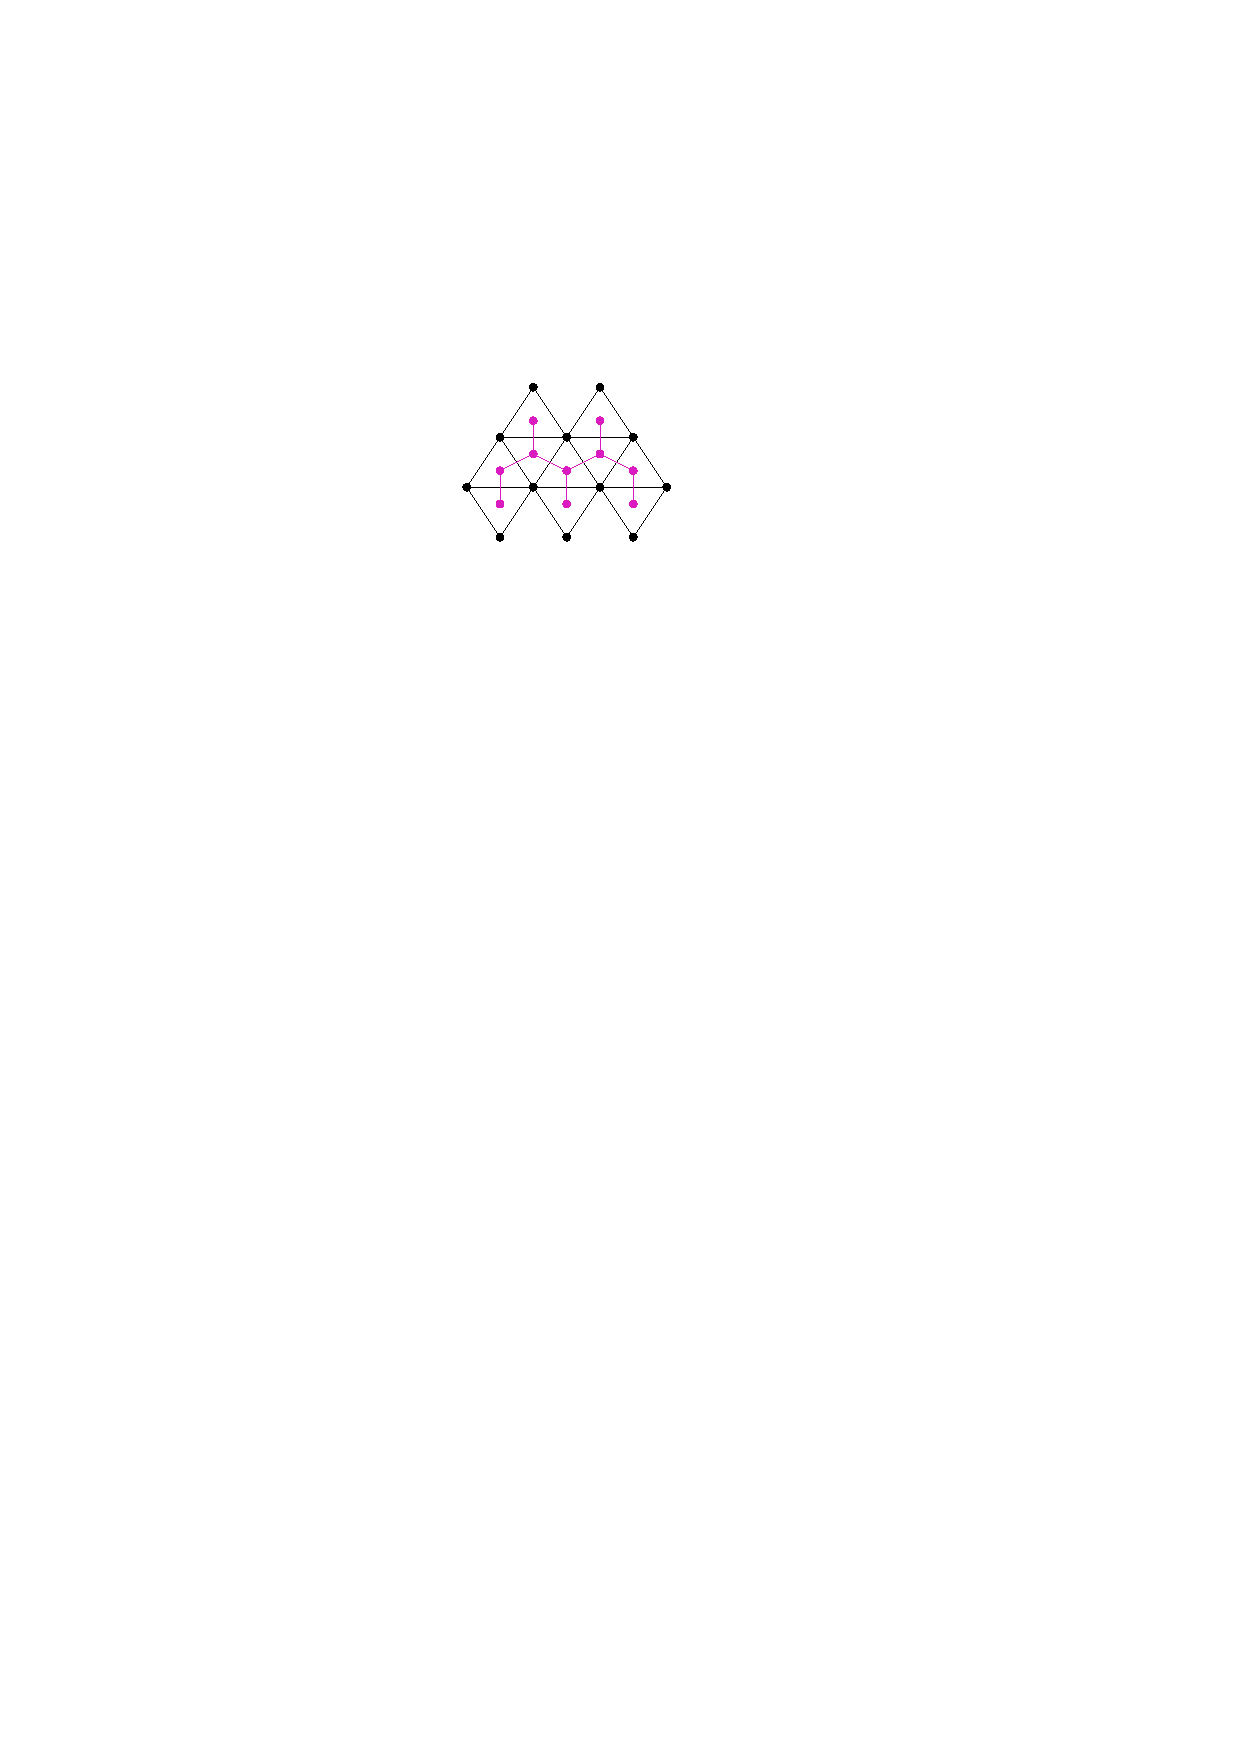
\includegraphics[page=1,width=0.7\linewidth]{graphics/maximal_outerplanar_extension_ratio.pdf}
		\caption{A straight-line drawing of a maximal outerplanar graph $G$ with its weak dual graph magenta-colored. The ratio is optimal}
	\end{subfigure}
	\begin{subfigure}{0.5\textwidth}
		\centering
		\includegraphics[page=2,width=0.7\linewidth]{graphics/maximal_outerplanar_extension_ratio.pdf}
		\caption{Extending $G$ results in a ratio increase due to area restrictions, colored in orange}
	\end{subfigure}
	\caption{Illustration of area restriction for dense maximal outerplanar graphs}
\end{figure}
This results in short euclidian distances relative to the longest edge, increasing the ratio.\\

\subsection{Drawing Algorithm For Complete Outerplanar Graphs With One Bend}
The first approach of a drawing algorithm addresses a ratio optimization for dense outerplanar graphs. These class of maximal outerplanar graphs are described with help of properties regarding the weak dual graph in the following way.
\begin{definition}\label{def:complete_maximal_outerplanar}
	A maximal outerplanar graph is called \emph{complete} if its weak dual graph $G'^*$ fulfills these properties:
	\begin{enumerate}
		\item The root vertex has exactly three children
		\item Every other inner node has exactly two children. In other words, the subtrees adjacent to the root vertex are complete binary trees of height $h-1$
	\end{enumerate}
\end{definition}
A given maximal outerplanar graph can be drawn by using a drawing algorithm for its weak dual graph. In section \ref{s:k-ary_trees}, the $k$-ary tree drawing algorithm produces a straight-line drawing in $\mathcal{O}(n^2 \log n)$ area with a ratio of $1+\varepsilon,\varepsilon>0$. The drawing algorithm \ref{al:k-ary_trees} can be used with a minor modification to draw the weak dual graph of any complete maximal outerplanar graph $G$, since $G'^*$ is a subtree of a $3$-ary tree with the same height.\\

\begin{algorithm}[H]
	\KwIn{A complete maximal outerplanar graph $G'$}
	\KwOut{Straight-line drawing $\Gamma_{G'^*}$ with nearly optimal ratio}
	\caption{\texttt{DrawOuterWeakDual($G'$)}}\label{al:drawouterweakdual}
	$G^* \gets$ weak dual graph of $G$ with minimal height\\
	$h \gets$ \texttt{height($G'^*$)}\\
	\texttt{root} $\gets$ $G'^*$.\texttt{root}\\
	\texttt{Draw(root)}\\
	\texttt{Draw\_$3$-ary\_Children(\texttt{root},$3^h$,1)}\\
	\For{\texttt{$v \in$ root.children}}{
		\texttt{Draw\_$2$-ary\_Children($v$,$2^{h-1}$,$h-1$)}
	}
	\Return $\Gamma$
\end{algorithm}

Algorithm \ref{al:drawouterweakdual} produces a nearly optimal straight-line drawing for the weak dual graph of a complete outerplanar graph $G'$. The resulting drawing $\Gamma_{G'^*}$ provides assistance to draw the complete outerplanar graph $G'$. Every vertex of $\Gamma_{G'^*}$ serves as an anchor point for the drawing of its corresponding face in $G'$.\\
Starting at the root of $G^*$, a triangle is drawn around the root in a way, that each edge of $G^*$ from the root to its three children crosses exactly one edge of the corresponding triangle face in $G'$. The vertices for the triangle are placed as follows. The first vertex lies above the already drawn root with an euclidian distance to the root sufficiently high in order to preserve planarity for the remaining drawing. The other two vertices are placed inbetween the two triangles defined by the root, its $\{\text{left, right}\}$ and middle children.\\
In order to guarantee a valid vertex and bend placement at every inner node $v^*$, the drawing is stretched horizontally and vertically by a factor of three.\\
Then, the drawing algorithm iterates over the height of $G'^*$. For every vertex $v^*$ of height $i\in \{1,...,h\}$ in $G'^*$, two bend points are placed 1 \UL left and right from $\Gamma_{G'^*}(v^*)$, and the new vertex $v$ is placed 1 \UL below from $\Gamma_{G'^*}(v^*)$.\\
$v^*$ is adjacent to an edge $e^*$ defined in $G^*$ that is crossing exactly one edge $e = (v_1,v_2)$ of $G'$. This crossing corresponds to the vertices defining the new face, $\{v, v_1, v_2\}$. Since $G'^*$ consists of three complete binary subtrees connected to the root, using the bends to draw the new face will preserve planarity since the coordinate of every inner node inherits its unique $x$ value by construction of algorithm \ref{al:complete_k-ary_tree}.
This drawing approach is summarized in the following algorithm.\\
\begin{algorithm}[H]
	\KwIn{Complete outerplanar graph $G'$}
	\KwOut{Polyline drawing $\Gamma_{G'}$ with one bend per edge and ratio $\mathcal{O}(\log n)$}
	\caption{\texttt{DrawCompleteOuterplanar($G'$)}}\label{al:complete_outerplanar}\label{algo:complete_outerplanar_graph_dual}
	$\Gamma \gets $ \texttt{DrawOuterWeakDual($G'$)}\\
	$h \gets$ \texttt{height($G'^*$)}\\
	\For{$v^* \in G'^*$}{
		$x(v^*) \gets 3\cdot x(v^*)$
	}
	\tcc{Draw the triangle face around the root of ${G'^*}$}
	$root \gets$ $\Gamma(G^*.\texttt{root})$\\
	$l \gets$ $\Gamma(G^*.\texttt{root.leftChild})$\\
	$m \gets$ $\Gamma(G^*.\texttt{root.middleChild})$\\
	$r \gets$ $\Gamma(G^*.\texttt{root.rightChild})$\\
	$v_1 \gets$ $\Gamma$.\texttt{PlaceVertex($x(root),y(root)+h\cdot 3^h$)}\\
	$v_2 \gets$ $\Gamma$.\texttt{PlaceVertex($\frac{x(root)+x(l)+x(m)}{3},\frac{y(root)+y(l)+y(m)}{3}$)}\\
	$v_3 \gets$ $\Gamma$.\texttt{PlaceVertex($\frac{x(root)+x(m)+x(r)}{3},\frac{y(root)+y(m)+y(r )}{3}$)}\\
	$\Gamma$.\texttt{DrawLineSegment($v_1,v_2$)}\\
	$\Gamma$.\texttt{DrawLineSegment($v_1,v_3$)}\\
	$\Gamma$.\texttt{DrawLineSegment($v_3,v_2$)}\\
	
	\tcc{Iterate over the height to draw the remaining vertices of $G'$}
	\For{$i \in [1..h]$}{
		\For{$v^* \in G^*$ with height $i$}{
			$b_l \gets$ $\Gamma$.\texttt{PlaceBendPoint($x(v^*) - 1,y(v^*)$)}\\
			$b_r \gets$ $\Gamma$.\texttt{PlaceBendPoint($x(v^*) + 1,y(v^*)$)}\\
			$v \gets$ $\Gamma$.\texttt{PlaceVertex($x(v^*),y(v^*)-1$)}\\
			$e^* \gets (v^*,\texttt{parent}(v^*))$\\
			$e \gets (v_1, v_2)$ edge intersecting $e^*$
			\tcp{w.l.o.g. $v_1$ ordered left of $v_2$}
			$\Gamma.$\texttt{DrawLineSegment($v,b_l$)}\\
			$\Gamma.$\texttt{DrawLineSegment($b_l,v_1$)}\\
			$\Gamma.$\texttt{DrawLineSegment($v,b_r$)}\\
			$\Gamma.$\texttt{DrawLineSegment($b_r,v_2$)}
		}
	}
	$\Gamma$\texttt{.delete($G'^*$)}\\
	\Return $\Gamma$
\end{algorithm}


\subsubsection{Analysis}

\begin{theorem}
	Every complete outerplanar graph $G'$ admits a polyline drawing $\Gamma_G$ on $\mathcal{O}(n^2 \log n)$ area with one bend per edge, preserving outerplanarity. The drawing is constructed in linear time and the ratio lies in $\mathcal{O}(\log n)$.
\end{theorem}

\begin{proof}
	The triangle around the root of $G^*$ consists of a vertex $v_1$ placed atop of the root vertex with distance $h\cdot r^h$ and two vertices $v_2,v_3$ placed at the centroids of the triangles defined by $\{\texttt{root,root.leftChild,root.middleChild}\}$ and $\{\texttt{root,root.middleChild,root.rightChild}\}$. By construction it holds, that $v_2$ and $v_3$ partition three binary subtrees rooted at the children of the root of $G'^*$ by their $x$ coordinate. The placement of the vertices $v_1,v_2$ and $v_3$ guarantee exactly one intersection between an edge of $G'$ and an edge of $G'^*$ in $\Gamma$.\\
	After stretching the drawing horizontally by a factor of three, there exist free grid points next to every vertex of $G^*$ which guarantees a grid point placement left and right of any vertex $v^*$. During the iteration over the height starting at height 1, every intersection between an edge of $G'^*$ and $G'$ refer to vertices on the outerface and a new face of $G'$ is attached on the outerface, preserving the outerplanarity of the drawing.\\
	Since $v_1$ is placed with a distance of $h\cdot r^h$ atop of the root of $G^*$ and $v_2$ and $v_3$ partition the $x$ coordinate of the binary subtrees rooted at the children of the root of $G^*$, planarity is preserved.\\
	The resulting area bounds are asymptotically the same compared to a drawing of a $3$-ary tree since the width and the height are multiplied by a constant. The area consumption lies still in $\mathcal{O}(n^2 \log n)$.\\
	The construction of $G'^*$ with minimal height lies in $\mathcal{O}(n)$ since there are $\mathcal{O}(n)$ faces for any maximal outerplanar graph. Drawing $G'^*$ and $G'$ lies in $\mathcal{O}(n)$. The runtime of this algorithm is therefore in linear time.\\
	The minimal euclidian distance values at least $2^h$ by construction of algorithm \ref{al:k-ary_trees} and lies in $\mathcal{O}(n)$. The length of the longest polyline spans the whole height of the drawing and lies in $\mathcal{O}(n \log n)$. The ratio lies therefore in $\mathcal{O}(\log n)$ since the height of $G^*$ lies in $\mathcal{O}(\log n)$.
\end{proof}
\subsubsection{Example Drawing}

	\begin{figure}[H]
	\centering
	\begin{subfigure}{\textwidth}
		\centering
		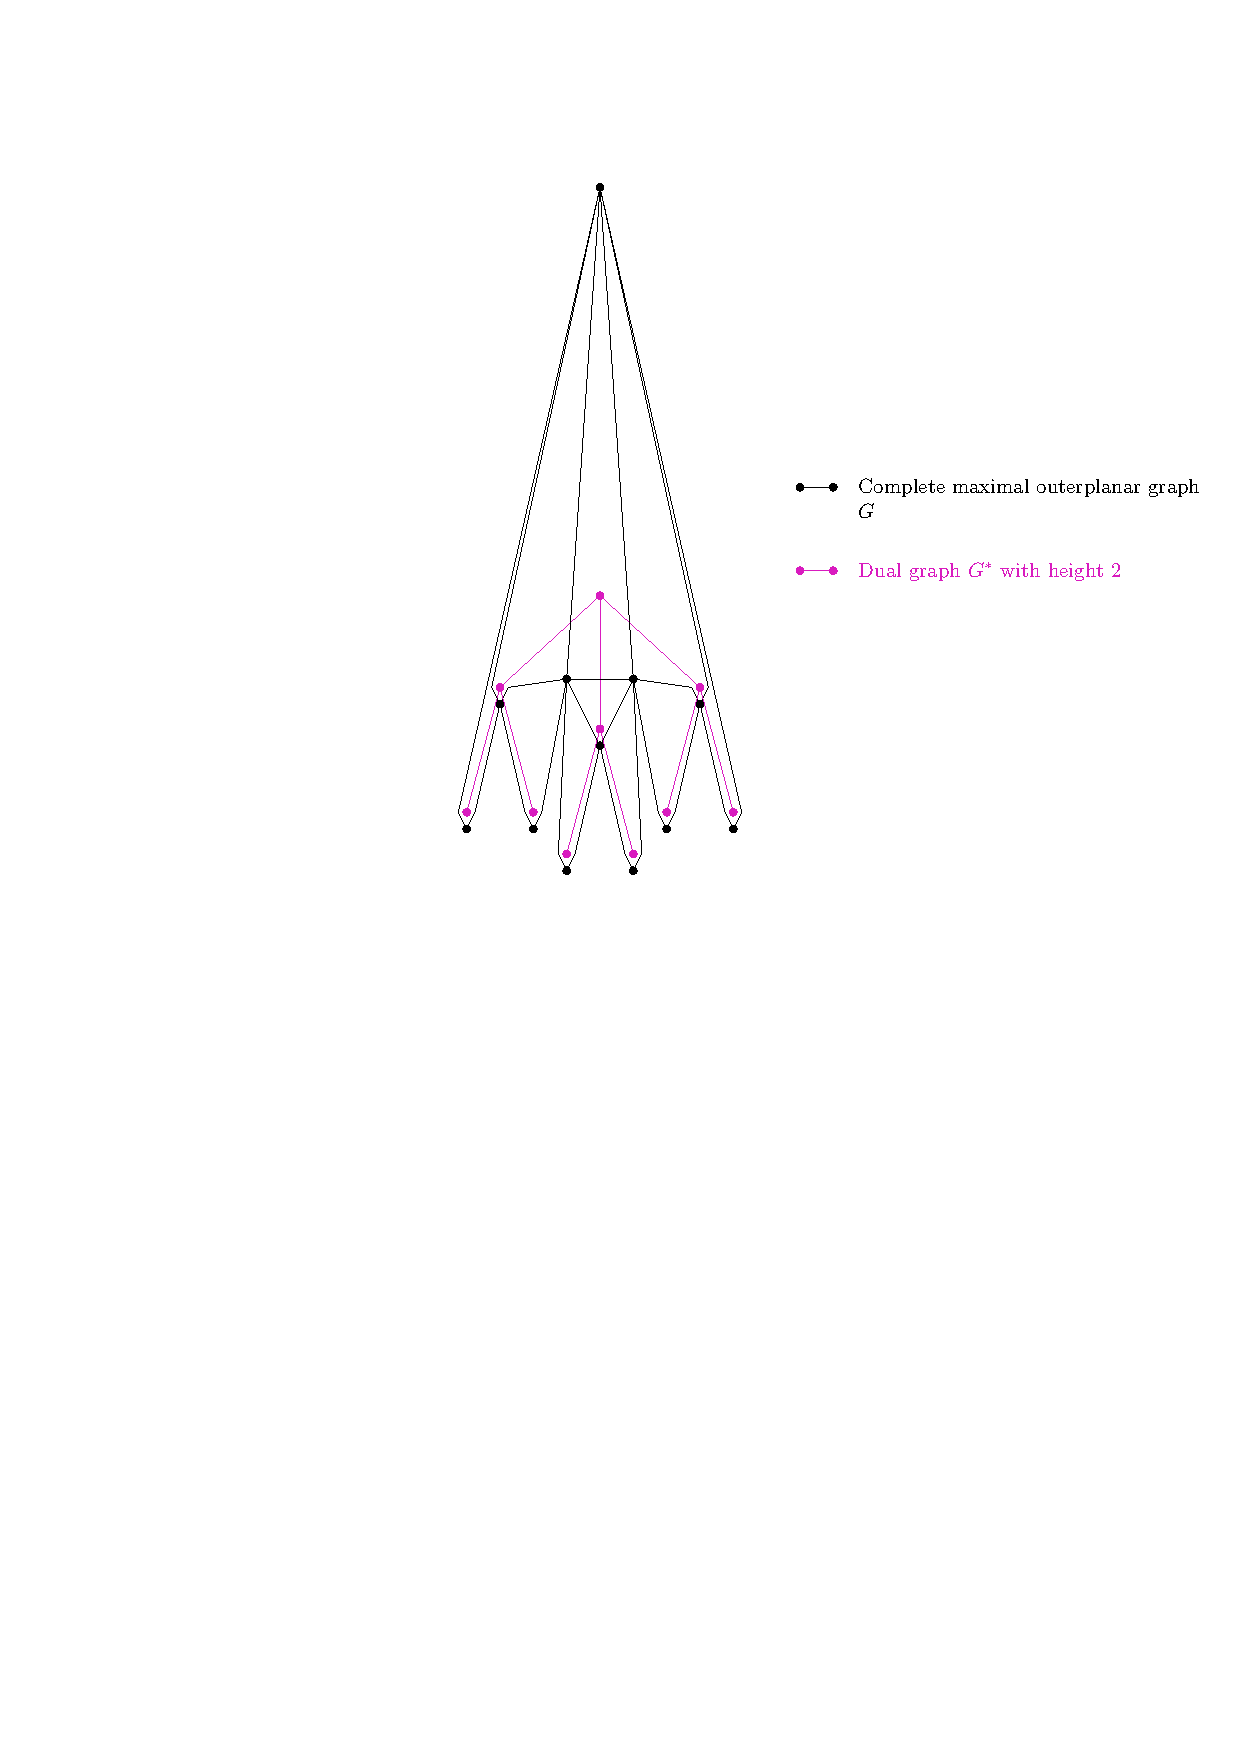
\includegraphics[page=1,width=0.7\linewidth]{graphics/complete_maximal_outerplanar_weak_dual_graph_example_drawing.pdf}
	\end{subfigure}
	\caption{Polyline drawing of a complete outerplanar graph $G'$. The dual graph $G'^*$ inherits a height of 2.}
\end{figure}


\subsubsection{Limitations}

As addressed by Observation \ref{ob:area_leads_to_ratio_increase}, this algorithm works fine for a complete maximal outerplanar graph $G'$ since then, the height of $G'^*$ is bound by $\mathcal{O}(\log n)$. On the other hand, when $G'$ is a loose maximal outerplanar graph, a height of $G^*$ might be of linear size and therefore, the drawing algorithm is not improving the ratio contrary to a straight-line drawing. In addition, the drawing algorithm will only work for simple weak dual graphs. The weak dual graph of a maximal SP graph is a multigraph.
	\begin{figure}[H]
	\centering
	\begin{subfigure}{\textwidth}
		\centering
		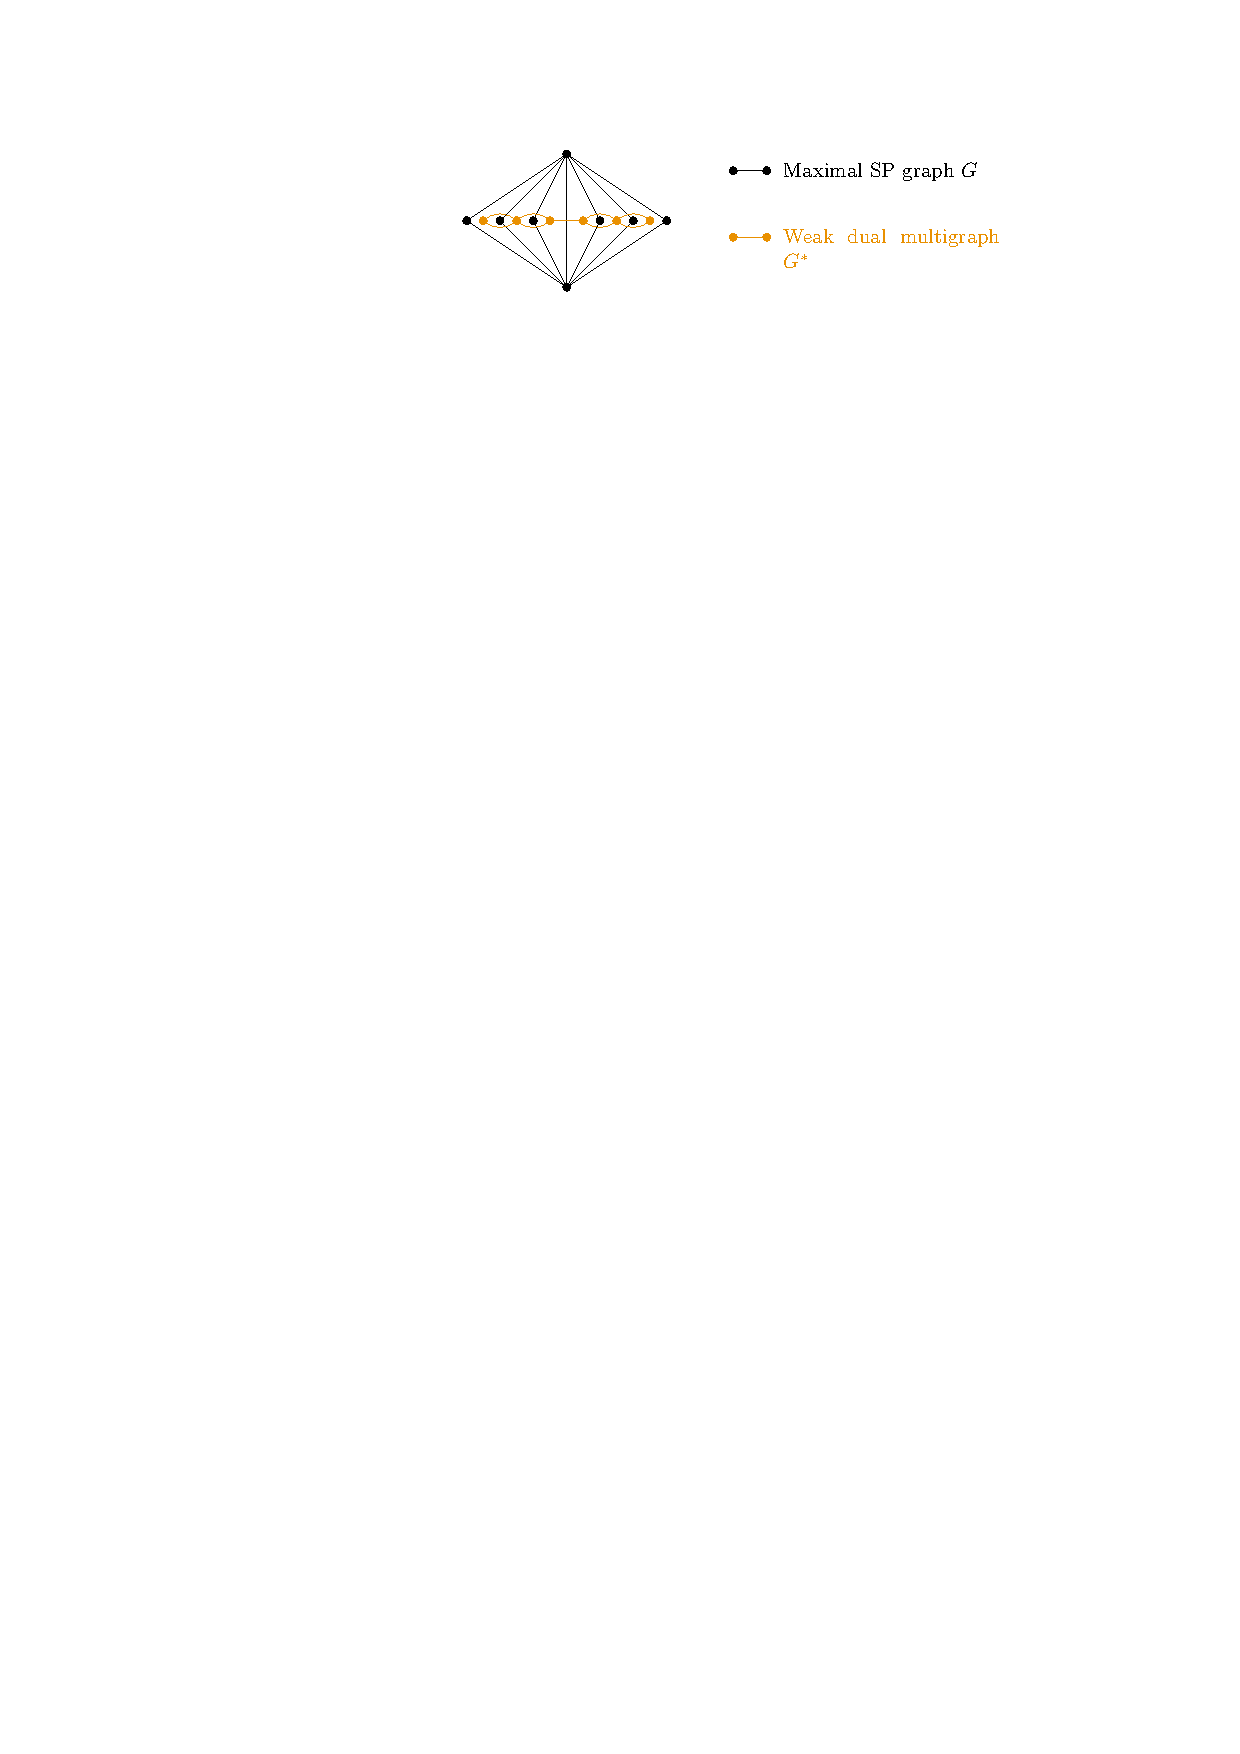
\includegraphics[page=1,width=0.6\linewidth]{graphics/maximal_sp_weak_dual.pdf}
	\end{subfigure}
	\caption{A maximal SP graph with its weak dual multigraph, colored in orange}
\end{figure}
The approach of drawing the weak dual graph at first followed by the outerplanar graph serves as an idea for a \emph{layered drawing}. The resulting drawings are valid layerings since the vertices of $G'$ added on a fixed height of $G'^*$ are not adjacent. As already observed, a layered drawing algorithm might guarantee a reasonable ratio by defining a minimal distance between two layers and therefore between two adjacent vertices. Since the weak dual graph is not suitable for 2-trees, the \emph{tree decomposition} of an SP-graph will serve as a guidance tool for the sequence of vertices drawn by a layering algorithm. The drawing algorithm will use the \emph{SPQR tree} derived from a tree decomposition.\\
When analyzing upper bounds for the ratio of a drawing for a maximal outerplanar graph $G'$, it is crucial to take a look at the tree structure of its tree decomposition. The following definition describes the difference of a $k$-ary tree $T$ to being a complete $k$-ary tree. This description of $k$-ary tree partitionings is very similar to a tree decomposition and will help during the analysis of a maximal outerplanar graph $G'$ with its tree decomposition, since any tree decomposition is a $k$-ary tree.
\subsection{Partitioning A $k$-ary Tree In Complete $k$-ary Subtrees}
\begin{definition}
	A \emph{partitioning} $P = (\mathcal{P},\mathcal{W})$ of a $k$-ary tree $T$ is defined with the following properties:
	\begin{itemize}
		\item For every vertex $p$ in $\mathcal{P}$ there exists a bag $w$ in $\mathcal{W}$
		\item Every bag $w$ in $\mathcal{W}$ contains a complete $k$-ary subtree of $T$ and is non-empty
		\item If there exists an edge in $T$ between two complete subtrees described by $w_1$ and $w_2$ out of $\mathcal{W}$, then $p_1$ and $p_2$ share an edge in $\mathcal{P}$
		\item $\mathcal{P}$ is a rooted tree		
	\end{itemize}
	A \emph{partition} is a pair consisting of a vertex of $\mathcal{P}$ and its corresponding bag $\mathcal{W}$. A partitioning $P$ is \emph{minimal} if every other partitioning $P'$ of $T$ contains a higher amount of partitions.
\end{definition}
Let $T$ be a $k$-ary tree with $n$ vertices. Then, for a partitioning $P$ covering all the vertices of $T$, the following holds:
\begin{enumerate}
	\item The amount of partitions of size $\mathcal{O}(1)$ is bound by $\mathcal{O}(n)$
	\item The amount of partitions of size $\mathcal{O}(\log n)$ is bound by $\mathcal{O}\left(\frac{n}{\log n}\right)$
	\item The amount of partitions of size $\mathcal{O}(\sqrt{n})$ is bound by $\mathcal{O}(\sqrt{n})$
	\item The amount of partitions of size $\mathcal{O}(n)$ is bound by $\mathcal{O}(1)$
\end{enumerate}
Also, any combination of partitions are possible. Presuming that a partitioning covers $\mathcal{O}(n)$ vertices of a graph, any combination of multiple partitionings of constant amount is possible. For example, let $|V(G')| = 2n$. One chain of $\mathcal{O}(n)$ vertices followed by a complete $k$-ary tree with $n$ vertices results in a legitimate $k$-ary tree with height $\mathcal{O}(n)$. The minimal partitioning of this example consists of $\mathcal{O}(n)$ partitions in total.
	\begin{figure}[H]
	\centering
	\begin{subfigure}{\textwidth}
		\centering
		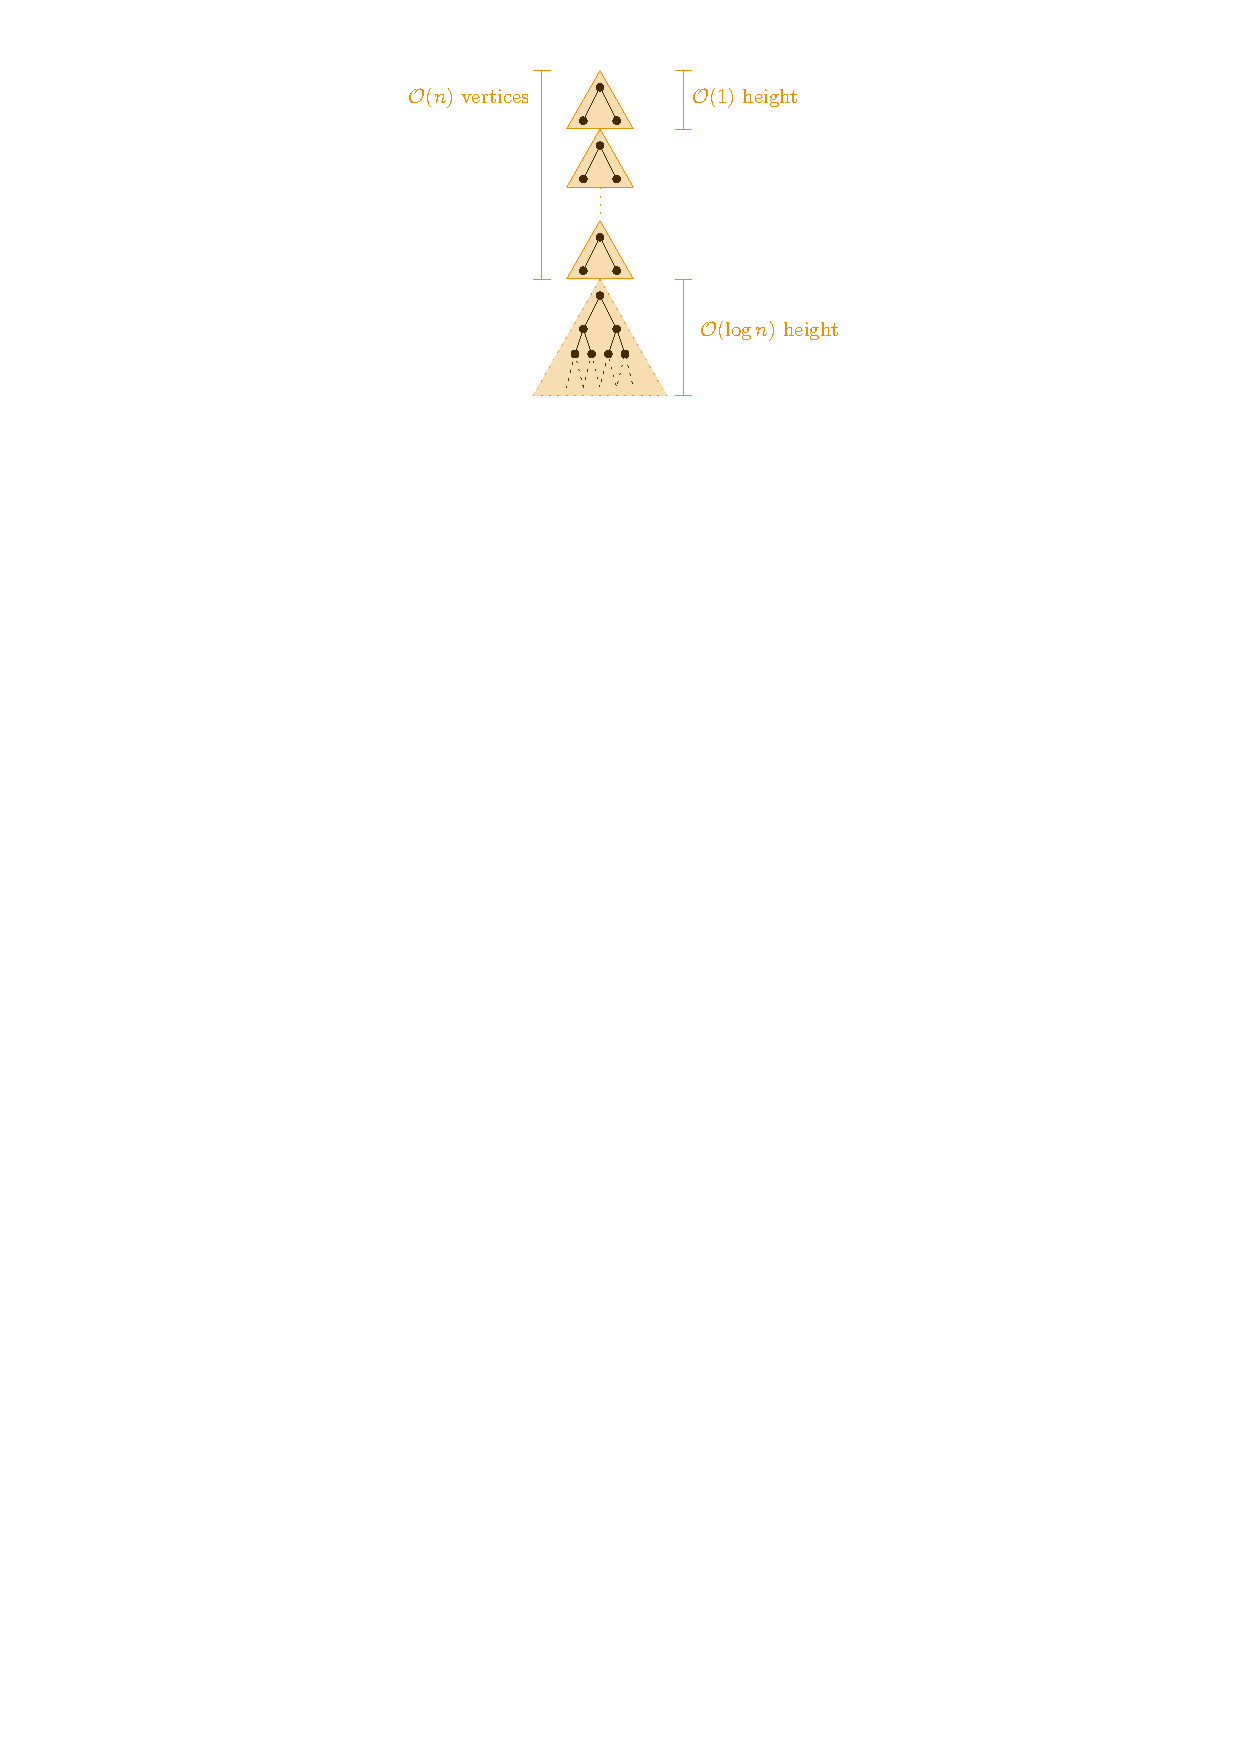
\includegraphics[page=1,width=0.7\linewidth]{graphics/k-ary_tree_partitioning_example.pdf}
	\end{subfigure}
	\caption{A $k$-ary tree of $\mathcal{O}(n)$ height partitioned in complete $k$-ary subtrees (in orange)}\label{im:partitioning_example}
\end{figure}


\begin{lemma}\label{l:partition_binary_tree_lower_upper_bounds}
	The height of $G$ interacts with the minimal partitioning $P$ of $G$ in the following way:
	\begin{enumerate}
		\item If $P$ consists of $\mathcal{O}(n)$ many partitions of constant size, the height of $G$ lies between $\Omega(\log n)$ and $\mathcal{O}(n)$
		\item If $P$ consists of $\mathcal{O}\left(\frac{n}{\log n}\right)$ partitions of size $\mathcal{O}(\log n)$, then the height of $G$ lies between $\Omega\left(\log\left(\frac{n}{\log n}\right)\cdot \log \log n \right)$ and $\mathcal{O}\left( n\right)$
		\item If $P$ consists of $\mathcal{O}(\sqrt{n})$ partitions of size $\mathcal{O}(\sqrt{n})$, then the height of $G$ lies between $\Omega(\log^2 n)$ and $\mathcal{O}(\sqrt{n}\log n)$
		\item if $P$ consists of a constant amount of partitions of size $\mathcal{O}(n)$, then the height is bound by $\mathcal{O}(\log n)$.
	\end{enumerate}
\end{lemma}
\begin{proof}
	Let $T$ be a $k$-ary tree and $P=(\mathcal{P},\mathcal{W})$ its minimal partitioning. Without loss of generality, it is presumed that all partitions of $P$ are of the same size. Since $\mathcal{P}$ is a tree, the following extremal cases for $\mathcal{P}$ are considered for the height of $T$:
	\begin{figure}[H]
		\centering
		\begin{subfigure}{0.6\textwidth}
			\centering
			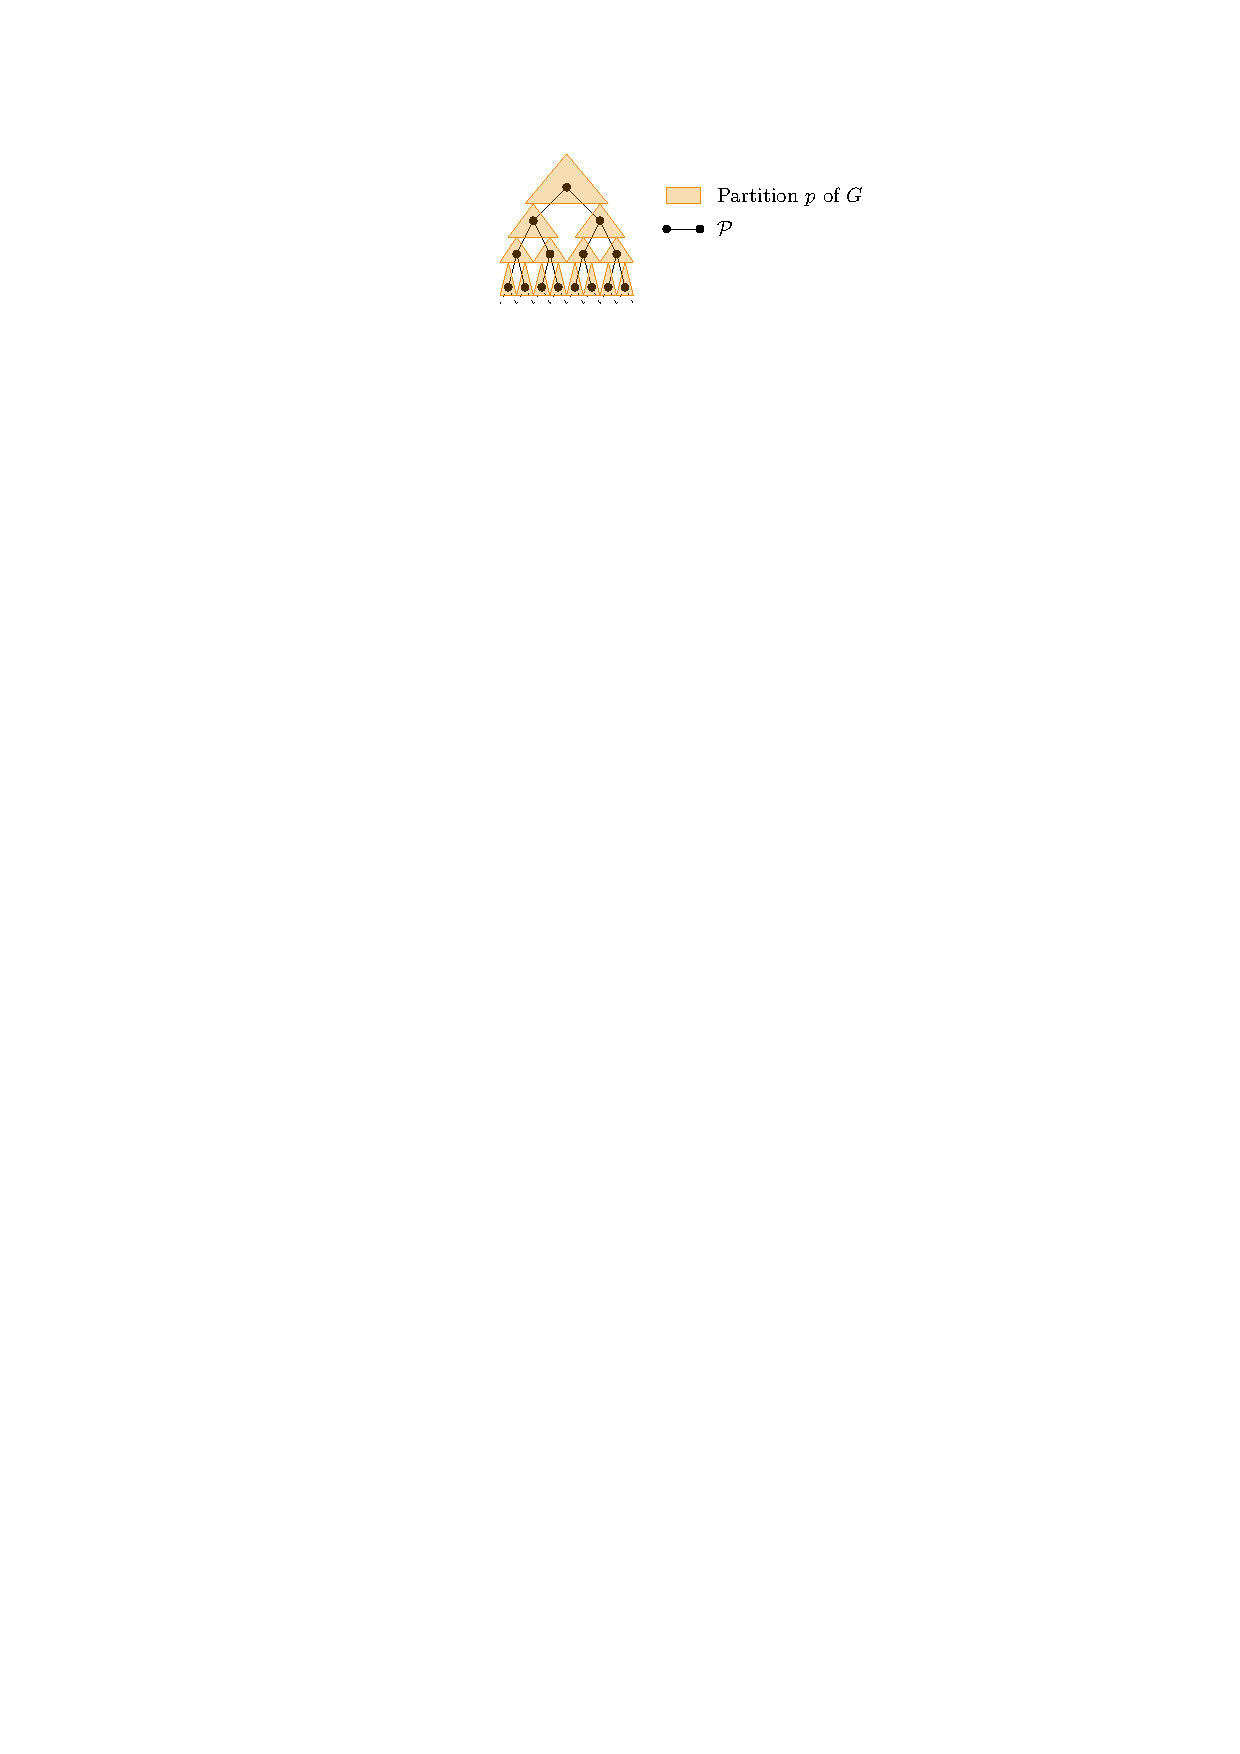
\includegraphics[page=1,width=\linewidth]{graphics/Partitioning_scheme.pdf}
			\caption{$\mathcal{P}$ represents a complete binary tree}\label{im:partitioning_binary}
		\end{subfigure}
		\begin{subfigure}{0.6\textwidth}
			\centering
			\includegraphics[page=2,width=\linewidth]{graphics/Partitioning_scheme.pdf}
			\caption{$\mathcal{P}$ represents a chain of vertices}\label{im:partitioning_chain}
		\end{subfigure}
		\caption{Extremal cases regarding the structure of $P$ of a partitioning $\mathcal{P}$}\label{im:partitioning_scheme}
	\end{figure}
	One extremal case covers $\mathcal{P}$ being a complete binary tree. By Lemma \ref{l:k-ary-tree_log_height}, for the height investigation of $G$ it suffices $\mathcal{P}$ to be binary since every complete $k$-ary tree has asymptotically the same height bound. The other extremal case covers a chain of vertices of $\mathcal{P}$. For case \ref{im:partitioning_binary}, $\mathcal{P}$ is a tree with height $\mathcal{O}(\log |\mathcal{P}|)$ and up to $\mathcal{O}(|\mathcal{P}|)$ height in case \ref{im:partitioning_chain}.
	\begin{enumerate}
		\item A complete $k$-ary tree of constant size inherits a constant height. With $|\mathcal{P}|\in \mathcal{O}(n)$, substituting every vertex of $\mathcal{P}$ with complete $k$-ary trees of constant height does not alter the height asymptotically and the height bounds are valid.
		\item A complete $k$-ary tree with $\mathcal{O}(\log n)$ vertices inherits a height of $\mathcal{O}(\log \log n)$. The height of $\mathcal{P}$ lies in $\mathcal{O}\left(\log\left(\frac{n}{\log n}\right)\right)$ for case \ref{im:partitioning_binary} and $\mathcal{O}\left(\frac{n}{\log n}\right)$ for case \ref{im:partitioning_chain}. Therefore, the height of $G$ lies in $\mathcal{O}\left(\log\left(\frac{n}{\log n}\right)\cdot \log \log n \right)$ for case \ref{im:partitioning_binary} and $\mathcal{O}\left(\frac{n}{\log n}\cdot \log \log n\right)$ for case \ref{im:partitioning_chain}.
		\item If every vertex of $\mathcal{P}$ represents a complete $k$-ary tree of height $\mathcal{O}(\log \sqrt{n}) = \mathcal{O}(\log n)$, the resulting total height of $G$ is in $\mathcal{O}(\log^2 n)$ for case \ref{im:partitioning_binary} and in $\mathcal{O}(\sqrt{n} \log n)$ for case \ref{im:partitioning_chain}. 
		\item A constant multiple of $\log n$ height for a vertex in $\mathcal{P}$ results in a total height of $\mathcal{O}(\log n)$ for $G$.
	\end{enumerate}
\end{proof}

\subsection{More Properties Of Maximal Outerplanar Graphs}

\begin{lemma}\label{l:outerplanar_tree_decomposition}
	Any maximal outerplanar graph $G'$ has a tree decomposition $(T',W')$ such that $T'$ is of degree at most 3.
\end{lemma}
\begin{proof}
	Consider the weak dual graph $G'^*$ considered in Definition \ref{def:complete_maximal_outerplanar}. For vertices $v_1^*,v_2^*$ in $G'^*$, insert vertices $t_1,t_2$ in $T$ which are adjacent if $v_1^*,v_2^*$ are adjacent in $G^*$. The corresponding bags $w_1, w_2$ contain the vertices of $G$ which define the face referred by $v_1^*,v_2^*$ in $G^*$. $T$ is isomorphic to $G^*$ and therefore is of degree at most 3.
\end{proof}


\begin{lemma}\label{l:outerplanar_two_vertices_subtree_TD_2}
	Let $v,w$ be any two adjacent vertices in a maximal outerplanar graph $G$. Then, the connected subtree $T'$ of a tree decomposition of $G$ containing both $v$ and $w$ contains at most two vertices.
\end{lemma}
\begin{proof}
	If $T'$ would contain at least 3 vertices, then there would exist three distinct vertices in $G$ forming a 3-clique with $v$ and $w$, destroying the outerplanarity property of $G$.
\end{proof}

\begin{lemma}\label{l:outerplanar_TD_properties}
	Let $(T,W)$ be the tree decomposition of a maximal outerplanar graph $G$, $t_1,t_2,t_p \in V(T)$ and $t_1, t_2$ are the children of $t_p$. Then, the following holds:
	\begin{enumerate}
		\item For $i = 1,2$, the bags $w_i$ and $w_p$ share exactly two vertices
		\item $w_1$ and $w_2$ share exactly one vertex
	\end{enumerate}
\end{lemma}
\begin{proof}
	\begin{enumerate}
		\item Since $G$ is a maximal outerplanar graph and therefore a 2-tree, all bags contain exactly 3 vertices. Since $t_p$ is the parent of $t_1$, their bags have two vertices in common when adding a vertex to two adjacent vertices of $t_p$.
		\item This follows directly by Lemma \ref{l:outerplanar_two_vertices_subtree_TD_2}.
	\end{enumerate}
\end{proof}

\begin{lemma}
	Let $(T,W)$ be a tree decomposition of a given maximal outerplanar graph $G$. The subtree $T'$ of $T$ containing a vertex $v$ of $G$ is a path and of length $\mathcal{O}(\texttt{height}(T))$.\label{l:max_outerplanar_active_vertex_path}
\end{lemma}
Let $t_p$ the parent of $t_1,t_2$ and $t_3$ and $v \in w_p$. Assume, that $v \in w_1,w_2,w_3$. Since the bags are of size three, there would be a vertex $v'\in w_p$ such that the subtree of $T$ containing $v,v'$ contains more than two vertices, contradicting Lemma \ref{l:outerplanar_two_vertices_subtree_TD_2}. Then, the subtree $T$ containing $v$ is of degree 2 and therefore a list.

\begin{definition}
	When traversing a tree decomposition $(T,W)_G$ of a graph $G$ with DFS, a vertex $v\in V(G)$ is called \emph{active} as soon as a vertex of the connected subtree $T'$ of $T$ containing $v$ in its bags is explored during DFS. A vertex $v\in V(G)$ is called \emph{finished} if $T'$ has been fully explored by DFS.
\end{definition}

\begin{lemma}
	Let $G'$ be a maximal outerplanar graph and $(T',W')$ its tree decomposition with $h_{T'}$ as height of $T'$. When using DFS as graph traversal for a drawing algorithm of $G'$, a vertex $v'$ of $G'$ is active for at least $\Omega(h_{t'})$ steps.\label{l:one_vertex_active_height}
\end{lemma}
\begin{proof}
	This follows directly by Lemma \ref{l:max_outerplanar_active_vertex_path}.
\end{proof}

\begin{lemma}\label{l:complete_maximal_outerplanar_log_n_active}
	Let $G'$ be a complete maximal outerplanar graph and $(T',W')$ its tree decomposition. When traversing $(T',W')$ by using DFS, there are at most $\mathcal{O}(\log n)$ vertices active simultaneously.
\end{lemma}
\begin{proof}
	Let $v' \in V(G')$ and $T'_{v'}$ be the subtree of $T'$, containing $v'$ in its bags. By Lemma \ref{l:one_vertex_active_height}, $T'_{v'}$ is a chain of vertices. Since $G'$ is maximal outerplanar, by Lemma \ref{l:outerplanar_two_vertices_subtree_TD_2} it holds that the amount of occurences of any other vertex $w'\in V(G')\setminus\{v'\}$ is bound by 2. Since $G'$ is complete, the height of $T'$ is bound by $\mathcal{O}(\log n')$.
		\begin{figure}[H]
		\centering
		\begin{subfigure}{\textwidth}
			\centering
			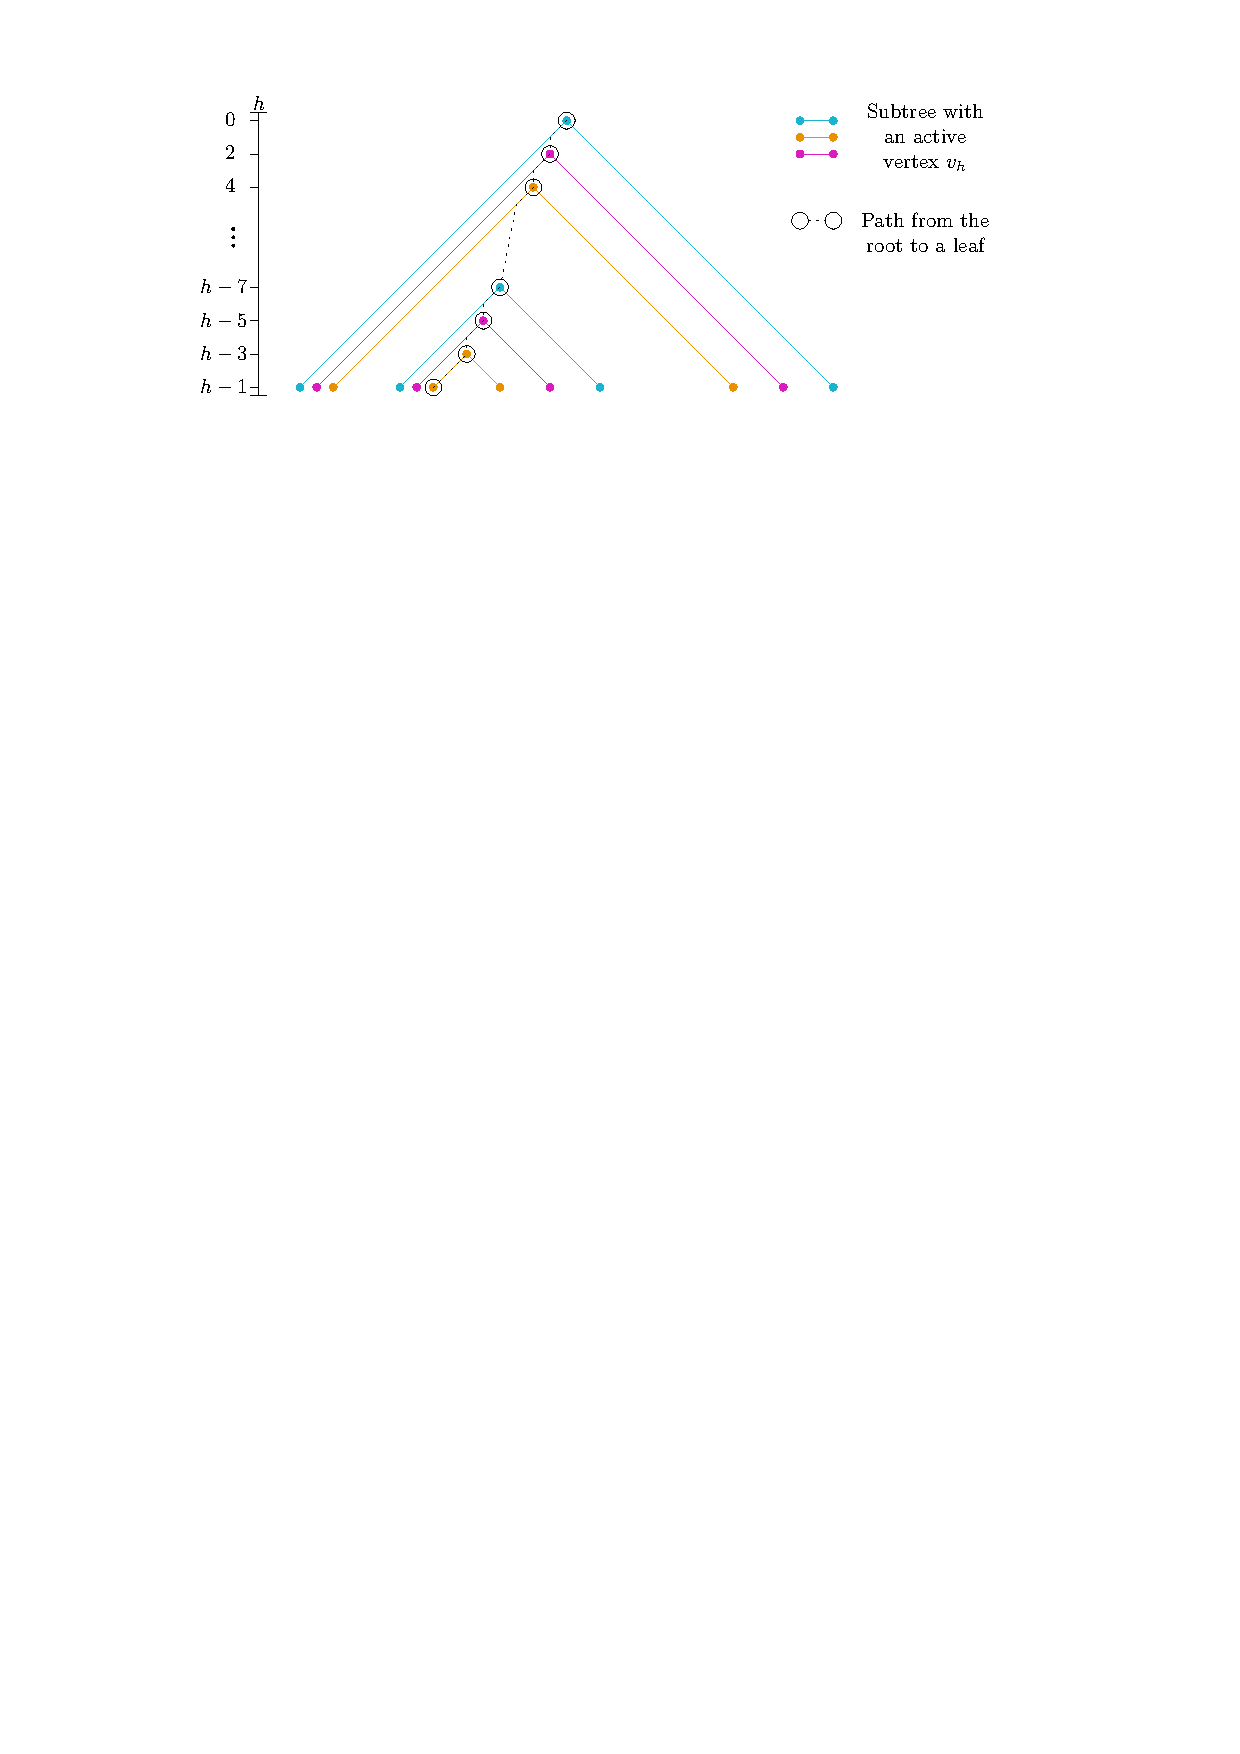
\includegraphics[page=1,width=0.9\linewidth]{graphics/active_vertices_log_n.pdf}
		\end{subfigure}
		\caption{A complete binary tree with up to $\mathcal{O}(\log n)$ active vertices for a DFS path}\label{im:active_vertices_log_n}
	\end{figure}

	Let $t'_r$ be the root and $t'_l$ a leaf of $T'$. Then, the path $p$ from $t'_r$ to $t'_l$ is unique. For every vertex $p_i$ of $p$, at most one vertex is set to being active during the DFS graph traversal, when starting at $t'_r$ up to $t'_l$. When $t'_l$ is explored, there are at most $\mathcal{O}(\log n')$ vertices still active. 
	The following holds for $p_i$ in $p$:
	\begin{itemize}
		\item If $p_i$ is a leaf and explored, then the induced new active vertex $v'_i\in V(G')$ is already finished since $|V(T'_{v'_i})| = 1$.
		\item If $p_i$ is not a leaf, then all the active vertices induced by exploring $p_{j}$ with $j>i$ are finished first when using DFS.
	\end{itemize}
	This means that up to $\mathcal{O}(\log n')$ vertices are active simultaneously when exploring $T'$.
\end{proof}

\begin{lemma}
	When prioritizing subtrees of minimal height while traversing any maximal outerplanar graph $G'$ with DFS, then there are up to $\mathcal{O}(\log^2 n')$ vertices active simultaneously.\label{l:maximal_outerplanar_log2_n_vercies_active}
\end{lemma}

\begin{proof}
	Let $G'$ be a maximal outerplanar graph with and $(T',W')$ be its tree decomposition. The height of $T'$ is bound by $\mathcal{O}(n')$. Since the degree of any vertex in $T'$ is at most 3, there are up to three binary trees connected to the root of $T'$. The minimal partitioning of the three binary subtrees $P_i = (\mathcal{T}_i,\mathcal{W}_i)$ of $T'$, $1\leq i \leq 3$, consist of binary tree partitions and $\mathcal{T}_i$ are binary trees.\\
	Consider a minimal partitioning $\mathcal{P}$ and a path $\tilde{t} = (t_1,...,t_k)$ starting at the root and ending at a leaf of $\mathcal{T}$. When subtrees of minimal heights are prioritized during every step of the DFS of $T$, then it holds that by the time the DFS reached a partition $t_j \in \tilde{t}$, then all the other partitions $t_i, i<j$ have been almost fully explored, leading to a constant amount of locally active vertices.\\
	In the case of $P$ being a complete binary tree, the priority of the subtree with the smallest height does not take any effect. Considering Lemma \ref{l:partition_binary_tree_lower_upper_bounds}, the largest upper bound for the height of $T$ lies in $\mathcal{O}(\log^2 n)$ when a minimal partitioning $P$ consists of $\sqrt{n'}$ partitions with $\sqrt{n'}$ vertices per partition bag and $\mathcal{T}$ being a complete binary tree. analogously to the proof of Lemma \ref{l:complete_maximal_outerplanar_log_n_active}, traversing a path from the root of $T$ to any leaf will set up to $\mathcal{O}(\log^2 n')$ vertices active.
\end{proof}

\subsection{Drawing Algorithm For Maximal Outerplanar Graphs With Two Bends}

Based on the fact that a layering induced by the drawing algorithm \ref{algo:complete_outerplanar_graph_dual} did improve the ratio for dense maximal outerplanar graphs, a new approach will create a box drawing with the layering property. Since every maximal outerplanar graph has triangles as interior faces, its treewidth is bound by 2.\\
In order to draw a maximal outerplanar graph $G$, its tree decomposition will be transferred to an $SPQR$-Tree. 

\begin{lemma}
	There exists a function $f: (T,W) \to \mathcal{T}$ which derives an $SPQR$-Tree out of a tree decomposition of a maximal SP-graph $G$ with the following properties:
	\begin{enumerate}
		\item There is no $R$ node in $\mathcal{T}$
		\item The skeleton of any serial node $S$ consists of exactly three vertices $s_1,s_2,s_3$
		\item The asymptotic height of $\mathcal{T}$ equals the asymptotic height of $T'$		
	\end{enumerate}\label{l:tree_decomp_to_SPQR}
\end{lemma}
\begin{proof}
	Let $G$ be an maximal SP-graph and $(T,W)$ its tree decomposition. Let $t_r$ be the root of $T$, representing a triangle of the vertices $v_1,v_2,v_3$. Its $SPQR$-Tree $\mathcal{T}$ consists of three $Q$ vertices, one for every edge of the triangle, one $S$ node and one $P$ node. $\mathcal{T}$ is illustrated in the figure below:
	\begin{figure}[H]
		\begin{subfigure}{0.4\textwidth}
			\centering
			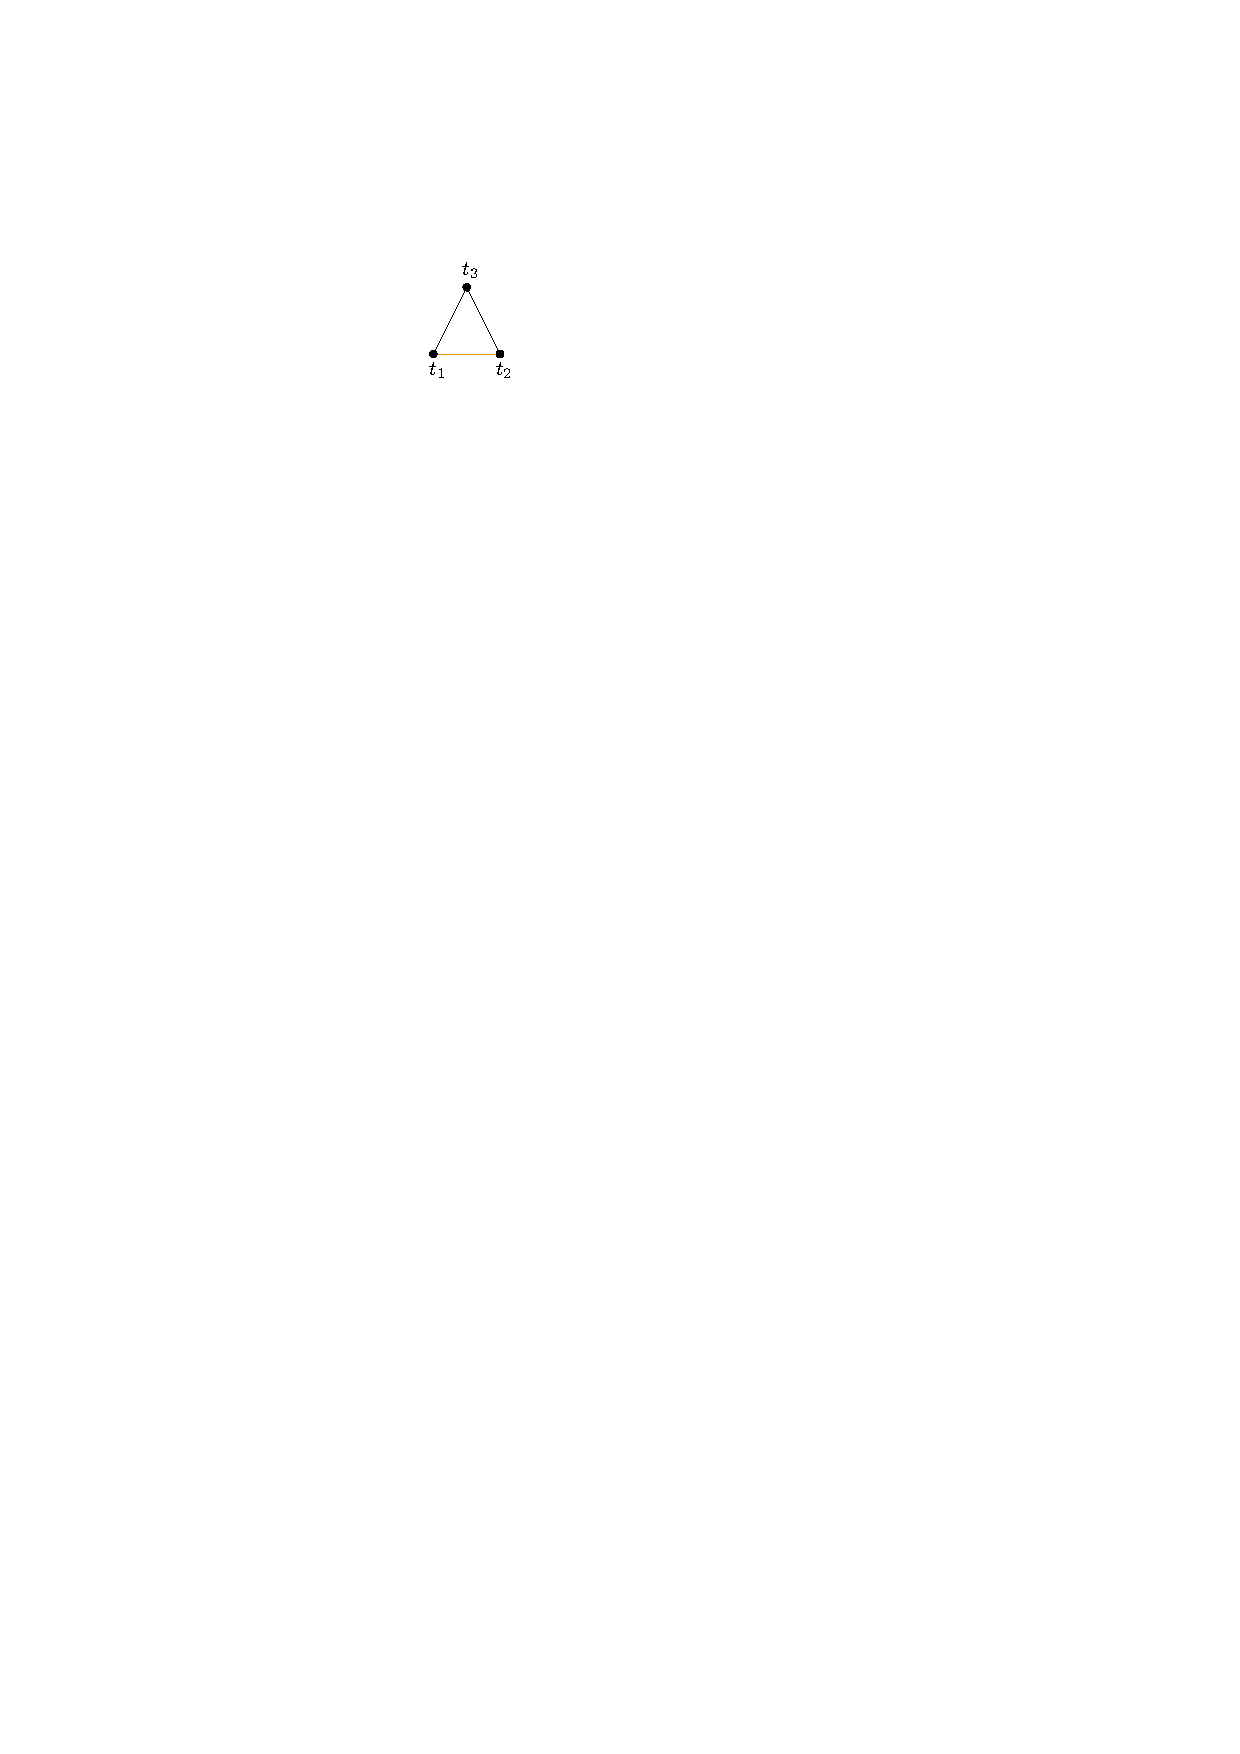
\includegraphics[page=1,width=0.7\linewidth]{graphics/SP_graphs_SPQR_inserting.pdf}
			\caption{A triangle}\label{im:SPQR_insert_a}
		\end{subfigure}
		\begin{subfigure}{0.4\textwidth}
			\centering
			\includegraphics[page=2,width=0.7\linewidth]{graphics/SP_graphs_SPQR_inserting.pdf}
			\caption{An $SPQR$-Tree of \ref{im:SPQR_insert_a}}\label{im:SPQR_insert_b}
		\end{subfigure}
		\caption{A triangle illustrated in figure \ref{im:SPQR_insert_a} and its $SPQR$-Tree in figure \ref{im:SPQR_insert_b}. The reference edge is marked in orange.}\label{im:SPQR_insert_1}
	\end{figure}
	When traversing $T$, every newly explored vertex of $T$ represents an addition of a new vertex of $G$ to $\mathcal{T}$. Let $v$ be the vertex of interest, adjacent to $v_1$ and $v_2$. $v_1$ and $v_2$ are already part of $\mathcal{T}$ and since the edge $(v_1,v_2)$ exists, there is a $Q$ node in $\mathcal{T}$ representing this edge. This $Q$ node is denoted as $Q(v_1,v_2)$. There are two cases to consider:
	\begin{description}
		\item[Case 1:] $Q(v_1,v_2)$ is adjacent to an $S$ node\\
		If $Q(v_1,v_2)$ is part of a serial composition in $\mathcal{T}$, adding $v$ will introduce a parallel composition around the split pair $(v_1,v_2)$ between $v$ and the residual graph $G\setminus\{v_1,v_2\}$. The following figure illustrates the insertion of $v$ into $\mathcal{T}$:
		\begin{figure}[H]
			\begin{subfigure}{\textwidth}
				\centering
				\includegraphics[page=3,width=\linewidth]{graphics/SP_graphs_SPQR_inserting.pdf}
			\end{subfigure}
			\caption{Insertion of a new vertex $v$ when $Q(v_1,v_2$ is not attached to a $P$ node)}\label{im:SPQR_insert_2}
		\end{figure}
		\item[Case 2:] $Q(v_1,v_2)$ is adjacent to $P(v_1,v_2)$\\
		Since there is already a parallel composition around the split pair $(v_1,v_2)$, inserting $v$ will be a serial composition as illustrated in the following figure:
		\begin{figure}[H]
			\begin{subfigure}{\textwidth}
				\centering
				\includegraphics[page=4,width=\linewidth]{graphics/SP_graphs_SPQR_inserting.pdf}
			\end{subfigure}
			\caption{Insertion of a new vertex $v$ when $Q(v_1,v_2$ is not attached to a $P$ node)}\label{im:SPQR_insert_2}
		\end{figure}
	\end{description}
	Since $G$ is a maximal SP-graph, there is not any $R$ node in $\mathcal{T}$ by definition. The second property holds as an invariant during the process of creating $\mathcal{T}$ since it is true for any triangle and any new vertex insertion. Every vertex of $T$ is substituted with a constant amount of vertices in $\mathcal{T}$, so the height of $\mathcal{T}$ equals the height of $T$ asympotically.\\
	So there exists a function $f$ which derives an $SPQR$-Tree from a given tree decomposition with the stated properties.
\end{proof}
The drawing algorithm will transfer a tree decomposition $(T',W')$ of a maximal outerplanar graph $G'$ to an $SPQR$-Tree $\mathcal{T}'$. Afterwards, the algorithm explores $\mathcal{T}'$ by DFS starting at the root node. This is achieved by a stack implementation in the pseudocode. For a vertex $t'\in V(\mathcal{T'})$, the child of $t'$ which roots the subtree of minimal height will always be prioritized during the DFS. This combined strategy of DFS and subtree priority will exclude unneccesarily inserted new layers in the resulting box drawing for $(T',W')$.\\
The following pseudocode creates a box drawing for a given $SPQR$-Tree:\\
\begin{algorithm}[H]
	\caption{\texttt{DrawSPQR}$(\mathcal{T})$}\label{al:maximal_outerplanar_box_two_bends}
	\label{al:draw_SPQR}
	\KwIn{$SPQR$-tree $\mathcal{T}$ of a graph $G$}
	\KwOut{Box drawing $\mathcal{B}_G$}
	Stack \texttt{stack}\\
	\texttt{SPQRVerticesDone} $\gets \emptyset$\\
	$v \gets \mathcal{T}.\texttt{root}$
	% \tcc{$\mathcal{T}$ is rooted at a $Q$ node with vertices $q_1, q_2$}
	\texttt{stack.push}$(\mathcal{T}.\texttt{root})$\\
	\texttt{column} $\gets 0$\\
	$\delta \gets $ pairwise distance between layers\\
	\texttt{Lower Layer} $l_{low} \gets 0$\\
	\texttt{Upper Layer} $l_{up} \gets l_{low} + \delta$\\
	% \tcc{$l_{low}, l_{up}$ describe layers of interest for the remaining drawing}
	$B.\texttt{DrawBox}(q_1, l_{up}, \texttt{column})$\\
	$B.\texttt{DrawBox}(q_2, l_{low}, \texttt{column})$\\
	$\texttt{ActiveVertices} \gets \{q_1,q_2\}$\\
	\While{\texttt{VerticesDone} $\neq V(\mathcal{T})$}{
		$v\gets \texttt{stack.pop}$\\
		List \texttt{children} $\gets v\texttt{.children}$\\
		\texttt{children.SortByHeightOfSubtreesDescending}\\
		% \tcc{Every child of a vertex in $\mathcal{T}$ roots a subtree with its respective height}
		\While{\texttt{children} $\neq \emptyset$}{
			\texttt{stack.push(head(children))}
			\texttt{children.remove(head(children))}
		}
		\If(\tcp*{$Q$ node refers an edge $(q_1,q_2)$ of $G$}){$v$ is $Q$ node}{
			$B$\texttt{.DrawEdge}$((q_1,q_2),\texttt{column})$\\
			\If{$q_1$ finished}{
				\texttt{ActiveVertices.remove}$(q_1)$
			}
			\If{$q_2$ finished}{
				\texttt{ActiveVertices.remove}$(q_2)$
			}
			
		}
		\ElseIf{$v$ is $P$ node}{
			$\texttt{column} \gets \texttt{column}+1$\\
			\For{$v\in \texttt{ActiveVertices}$}{
				$B\texttt{.extendBox}(v)$
			}
			$l_{up} \gets layer(p_1)$\\
			$l_{low} \gets layer(p_2)$
		}
		\ElseIf(\tcp*{Serialization $S(s_1,s_2,s_3)$}){$v$ is $S$ node}{
			$\texttt{column} \gets \texttt{column}+1$\\
			\For{$v\in \texttt{ActiveVertices}$}{
				$B\texttt{.extendBox}(v)$
			}
			\If{$\nexists$ free layer between $layer(s_1)$ and $layer(s_3)$}{$l \gets B$\texttt.{addLayer}$(l_{up},l_{low})$}
			\Else{$l \gets $ free layer between $layer(s_1)$ and $layer(s_3)$}
			$B\texttt{.DrawBox}(s_2, l)$\\
			$\texttt{ActiveVertices.add}(s_2)$
		}
		\texttt{VerticesDone.add}$(v)$
	}
\end{algorithm}
The whole strategy is summed up in the following pseudocode:\\
\begin{algorithm}[H]
	\caption{\texttt{DrawMaximalOuterplanar}($G'$)}\label{al:maximal_outerplanar_two_bends}
	\KwIn{Maximal Outerplanar Graph $G'$}
	\KwOut{Polyline drawing $\Gamma_{G'}$ with two bends}
	$(T,W) \gets$ tree decomposition of $G'$ with lowest height\\
	$\mathcal{T'} \gets f(T',W')$\\
	$\delta \gets n$\\
	$\mathcal{B}_{G'} \gets \texttt{DrawSPQR}(\mathcal{T'})$\\
	$\Gamma_{G'} \gets \mathcal{B}_{G'}.\texttt{TransferToPolyline}$\\
	\Return $\Gamma_{G'}$
\end{algorithm}

\subsubsection{Analysis}

Algorithm \ref{al:maximal_outerplanar_two_bends} takes a maximal outerplanar graph $G'$ as input argument. Calculating the tree decomposition of $G'$ with lowest height runs in $\mathcal{O}(n)$ time since there are $\mathcal{O}(n)$ faces in $G'$. Transferring the tree decomposition to an $SPQR$-Tree described by the function of Lemma \ref{l:tree_decomp_to_SPQR} takes $\mathcal{O}(|V(T')|) = \mathcal{O}(n)$ steps.\\
The drawing step described in Algorithm \ref{al:draw_SPQR} takes the $SPQR$-Tree and creates a box drawing by iterating over its nodes. For the $SPQR$-Tree $\mathcal{T}$, there are $\mathcal{O}(n)$ $P$, $S$ and $Q$ nodes, respectively. In case of a $Q$ node, drawing an edge takes constant time. In case of either a $P$ or a $S$ node, there are $\mathcal{O}(|\texttt{ActiveVertices}|)$ box extensions.\\
Transferring a box drawing to a polyline drawing includes the substitution of $\mathcal{O}(n)$ boxes with a grid point and $\mathcal{O}(n)$ edge reroutes over two bends per edge. The runtime therefore equals $\mathcal{O}(n\cdot |\texttt{ActiveVertices}|)$.

\begin{theorem}
	Let $G'$ be a complete maximal outerplanar graph. The drawing algorithm \ref{al:maximal_outerplanar_two_bends} produces a polyline drawing $\Gamma_{G'}$ on area $\mathcal{O}(n'^2 \log n')$ with two bends per edge and ratio $r \in \mathcal{O}(\log n')$, when the minimal distance between two layers is set to $n'$.\label{th:complete_maximal_outerplanar_ratio_logn}
\end{theorem}
\begin{proof}
	Consider the drawing algorithm \ref{al:maximal_outerplanar_box_two_bends}, producing a box drawing $\mathcal{B}_{G'}$. The algorithm first creates a tree decomposition of $G'$, $(T',W')$, and then uses DFS on $T'$ in its iteration to explore new active vertices which will be drawn in a potentially new layer. An active vertex $v$ blocks a layer of $\mathcal{B}_{G'}$ for further vertex insertions. When the DFS finished exploring the subtree $T'_{v}$ of $T'$, the layer of $v$ is availiable for new vertex insertions.\\
	Let $p$ be a path from the root of $T'$ to a leaf which creates the highest amount of layers. By Lemma \ref{l:complete_maximal_outerplanar_log_n_active}, there are up to $\mathcal{O}(\log n)$ vertices active during the DFS graph traversal of the tree decomposition of $G'$. Since $T'_{v}$ is a chain of vertices for any vertex $v\in V(G')$, there exists a subtree of $T'$ of asymptotically the same height as $T'_{v}$ which does not contain $v$ in its bags. After drawing $\mathcal{O}(\log n)$ vertices defined by $p$ on separate layers, the amount of layers created in $\mathcal{B}_{G'}$ suffice for the remaining drawing and is asympotitcally bound by $\mathcal{O}(\log n)$.\\
	The resulting box drawing therefore inherits $\mathcal{O}(\log n)$ layers with a pairwise distance of $n$. The height of the drawing is bound by $\mathcal{O}(n \log n)$. Since for every edge of $G'$ there exists a column in $\mathcal{B}_{G'}$, the width is bound by $O(n)$. The total area consumption therefore lies in $\mathcal{O}(n^2 \log n)$.\\
	When transferring the box drawing $\mathcal{B}_{G'}$ to a polyline drawing $\Gamma_{G'}$, every box $b_v$ is substituted with a grid point $v$ inside of $b_v$ and every edge incident to $b_v$ is rerouted by a bend point to the grid point for $v$. The polyline drawing produced by algorithm \ref{al:maximal_outerplanar_two_bends} inherits two bends per edge and has asymptotically the same area bound as the box drawing of algorithm \ref{al:maximal_outerplanar_box_two_bends}. The longest edge $l_{\max}$ spans the width and the height and its length is bound by $\mathcal{O}(n \log n) + \mathcal{O}(n) = \mathcal{O}(n \log n)$. The minimal Euclidian distance between to adjacent vertices values $n$ implied by the layering with its distance and the ratio therefore lies in $\mathcal{O}(\log n)$.
\end{proof}

\begin{theorem}
	Let $G'$ be a maximal outerplanar graph. The drawing algorithm \ref{al:maximal_outerplanar_two_bends} produces a polyline drawing $\Gamma_{G'}$ on area $\mathcal{O}(n'^2 \log^2 n')$ with two bends per edge and ratio $r \in \mathcal{O}(\log^2 n')$, when the minimal distance between two layers is set to $n'$.\label{th:maximal_outerplanar_log2_n_ratio}
\end{theorem}
\begin{proof}
	Considering Lemma \ref{l:maximal_outerplanar_log2_n_vercies_active}, up to $\mathcal{O}(\log^2 n')$ are active simultaneously when traversing the tree decomposition of $G'$ with DFS and prioritizing the subtrees of minimal height. Analouguously to the proof of Theorem \ref{th:complete_maximal_outerplanar_ratio_logn}, there are up to $\mathcal{O}(\log^2 n')$ layers inserted into the box drawing which will suffice for the whole drawing of $G'$. After transferring the box drawing to a polyline drawing, the resulting height lies in $\mathcal{O}(n\log^2 n)$. The width still lies in $\mathcal{O}(n)$. The ratio is therefore bound by $\mathcal{O}
	(\log^2 n')$. 
\end{proof}

\begin{theorem}
	There exists a class of maximal outerplanar graphs for which every graph admits a polyline drawing on $\mathcal{O}(n^2)$ area with a constant ratio.
\end{theorem}
\begin{proof}
	Let $G'$ be a maximal outerplanar graph with its partitioning $P = (\mathcal{P},\mathcal{W})$. Let $c$ be a constant so that for every partition $p_i \in \mathcal{P}$ it holds that $|w_i|\leq c, w_i \in \mathcal{W}$ and $\mathcal{P}$ be a chain of vertices of height $\mathcal{O}(n)$. Since the size of every partition is bound by $c$, the height of the regarding complete $k$-ary tree is bound by $\mathcal{O}(1)$.\\
	When $\mathcal{P}$ is a chain of vertices, the drawing algorithm \ref{al:maximal_outerplanar_two_bends} finishes a partition before proceeding to the next element of $\mathcal{P}$ due to the combined strategy of DFS and subtree priority. Since the amount of layers inserted into $\mathcal{B}_{G'}$ are determined by the amount of simultaneously active vertices, $\mathcal{B}$ inherits a constant amount of layers, resulting in a box drawing of $\mathcal{O}(n^2)$ area and a constant ratio.
\end{proof}
\newpage
\subsubsection{Example Drawing}

\begin{figure}[H]
	\centering
	\begin{subfigure}{\textwidth}
		\centering
		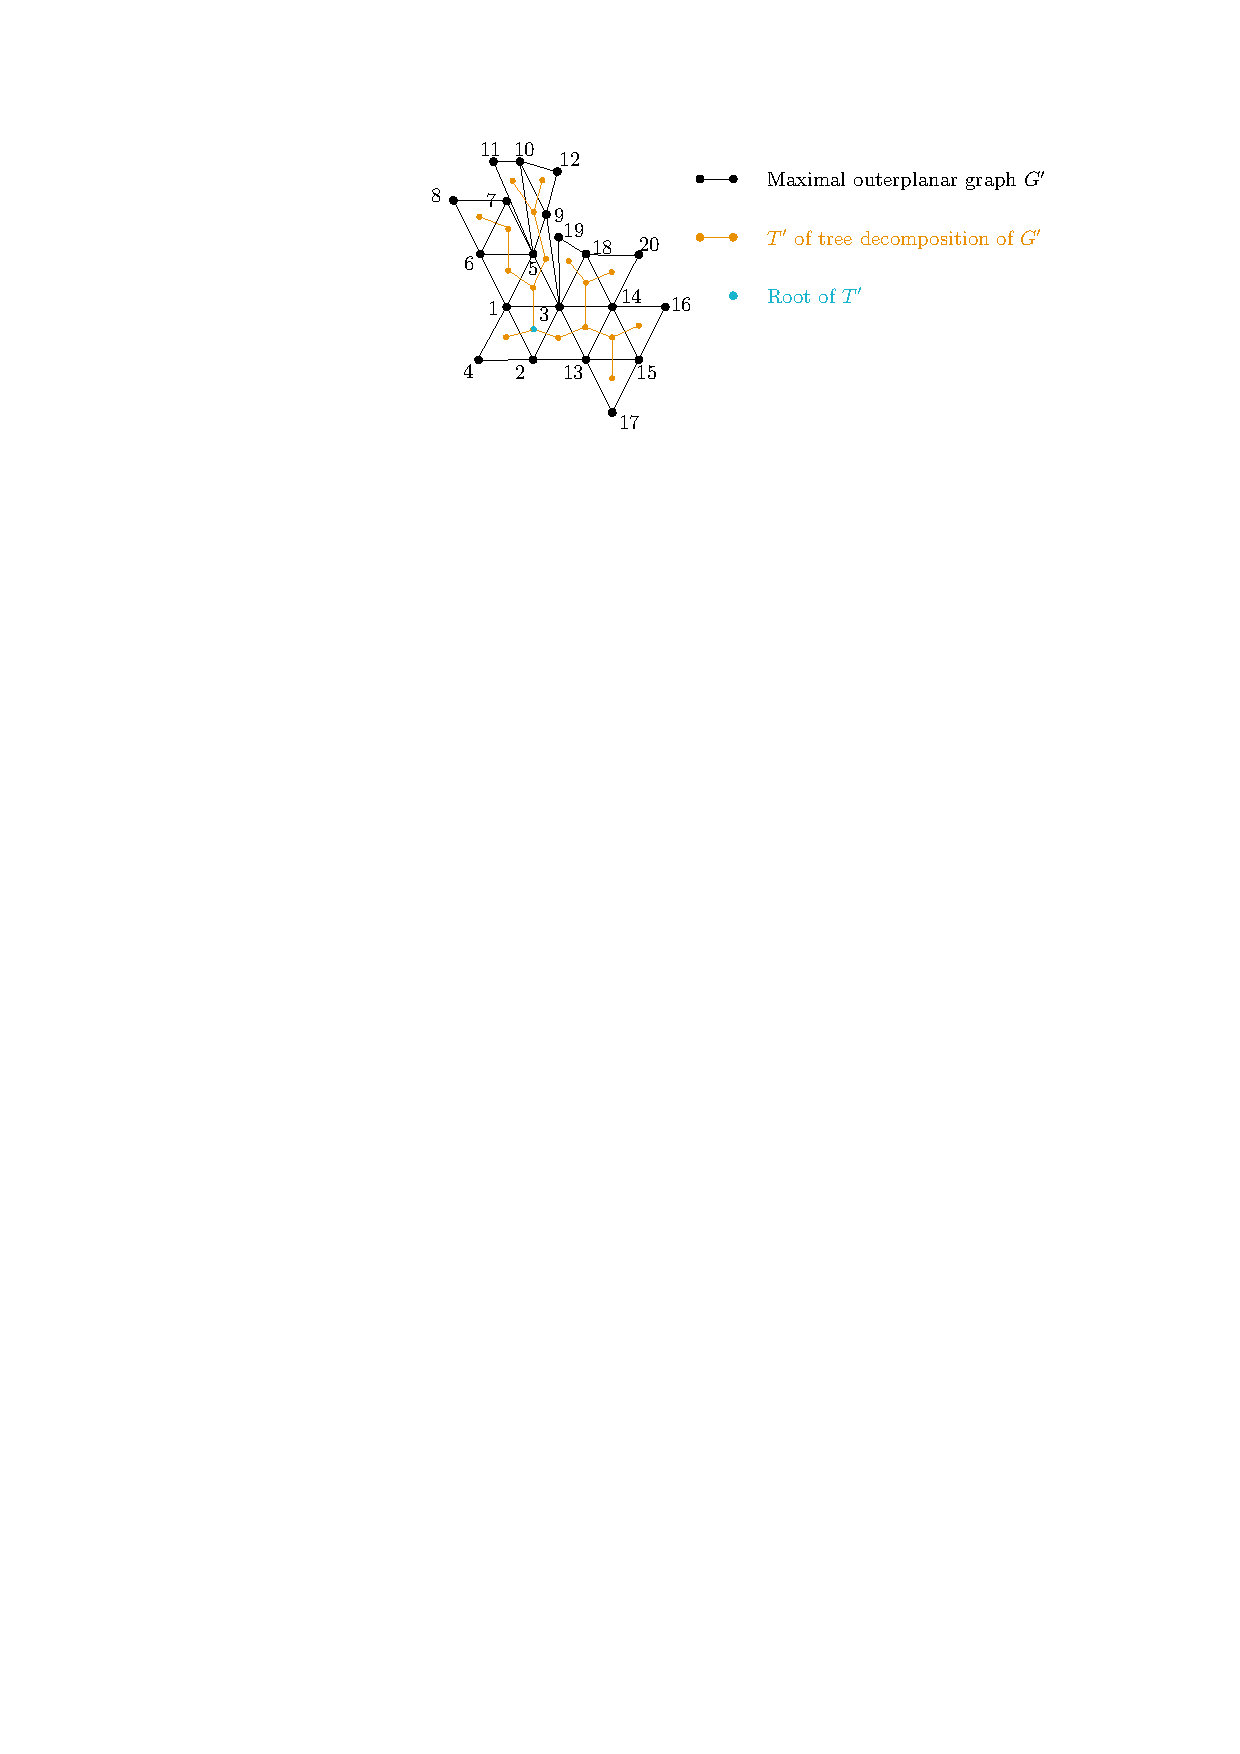
\includegraphics[page=1,width=0.9\linewidth]{graphics/maximal_outerplanar_example_drawings.pdf}
	\end{subfigure}
	\caption{A straight-line drawing of a maximal outerplanar graph $G'$ with $T'$ out of its tree decomposition}\label{im:maximal_outerplanar_example_straight-line}
\end{figure}
The drawing algorithm draws the triangle defined vertices $1,2$ and $3$ on three different layers and then explores $T'$ by DFS und prioritizes the subtree of minimal height. In the illustration of $T'$, the magenta enclosure illustrates the progression of the DFS.\\
In order to illustrate an example drawing properly, the distance between layers $\delta$ is set to 4.
\begin{figure}[H]
	\centering
	\begin{subfigure}{0.49\textwidth}
		\centering
		\includegraphics[page=2,width=\linewidth]{graphics/maximal_outerplanar_example_drawings.pdf}
		\caption{Box drawing $\mathcal{B}$ of the triangle $T(1,2,3)$}
	\end{subfigure}
\begin{subfigure}{0.49\textwidth}
\centering
\includegraphics[page=3,width=\linewidth]{graphics/maximal_outerplanar_example_drawings.pdf}
\caption{Inserting vertex $4$ into $\mathcal{B}$}
\end{subfigure}
\end{figure}
\begin{figure}[H]
	\centering
	\begin{subfigure}{\textwidth}
		\centering
		\includegraphics[page=5,width=0.7\linewidth]{graphics/maximal_outerplanar_example_drawings.pdf}
	\end{subfigure}
	\caption{After drawing vertex $6$, vertex 1 is finished and the vertices 6 to 8 alternate between two layers}
\end{figure}

\begin{figure}[H]
	\centering
	\begin{subfigure}{\textwidth}
		\centering
		\includegraphics[page=6,width=0.7\linewidth]{graphics/maximal_outerplanar_example_drawings.pdf}
	\end{subfigure}
	\caption{The subtree adjacent to vertices $5$ and $3$ is drawn}
\end{figure}

\begin{figure}[H]
	\centering
	\begin{subfigure}{\textwidth}
		\centering
		\includegraphics[page=7,width=0.7\linewidth]{graphics/maximal_outerplanar_example_drawings.pdf}
	\end{subfigure}
	\caption{The subtree adjacent to vertices $2$ and $3$ is drawn}\label{im:example_drawing_box_G}
\end{figure}


\begin{figure}[H]
	\centering
	\begin{subfigure}{\textwidth}
		\centering
		\includegraphics[page=8,width=0.5\linewidth]{graphics/maximal_outerplanar_example_drawings.pdf}
	\end{subfigure}
	\caption{The resulting polyline drawing $\Gamma_{G'}$ derived from $\mathcal{B}_{G'}$, with two bends per edge}\label{im:example_drawing_gamma_G}
\end{figure}
\subsubsection{Preserving Outerplanarity}

\begin{theorem}
	There exists an alternation of Algorithm \ref{al:draw_SPQR} that preserves the outerplanarity property of $\mathcal{G'}$ in a resulting box drawing $\mathcal{B}_{G'}$.
\end{theorem}
\begin{proof}
Start at the root of $T'$, drawing a triangle on three layers. Without loss of generality, let $v_1$ be on the top layer, $v_2$ on the bottom layer and $v_3$ inbetween, placed left of the edge $(v_1,v_2)$.
Since $G'$ is maximal outerplanar, by Lemma \ref{l:outerplanar_TD_properties} the three binary subtrees adjacent to the root of $T'$ address either $(v_1,v_2)$, $(v_1,v_3)$ or $(v_2,v_3)$. If a binary subtree refers to $(v_1,v_3)$, draw to the left inbetween the regarding layers. Analouguously for the binary tree referring to $(v_2,v_3)$. If a binary subtree refers the edge $(v_1,v_2)$, draw to the right. 
	
\begin{figure}[H]
	\begin{subfigure}{\textwidth}
		\centering
		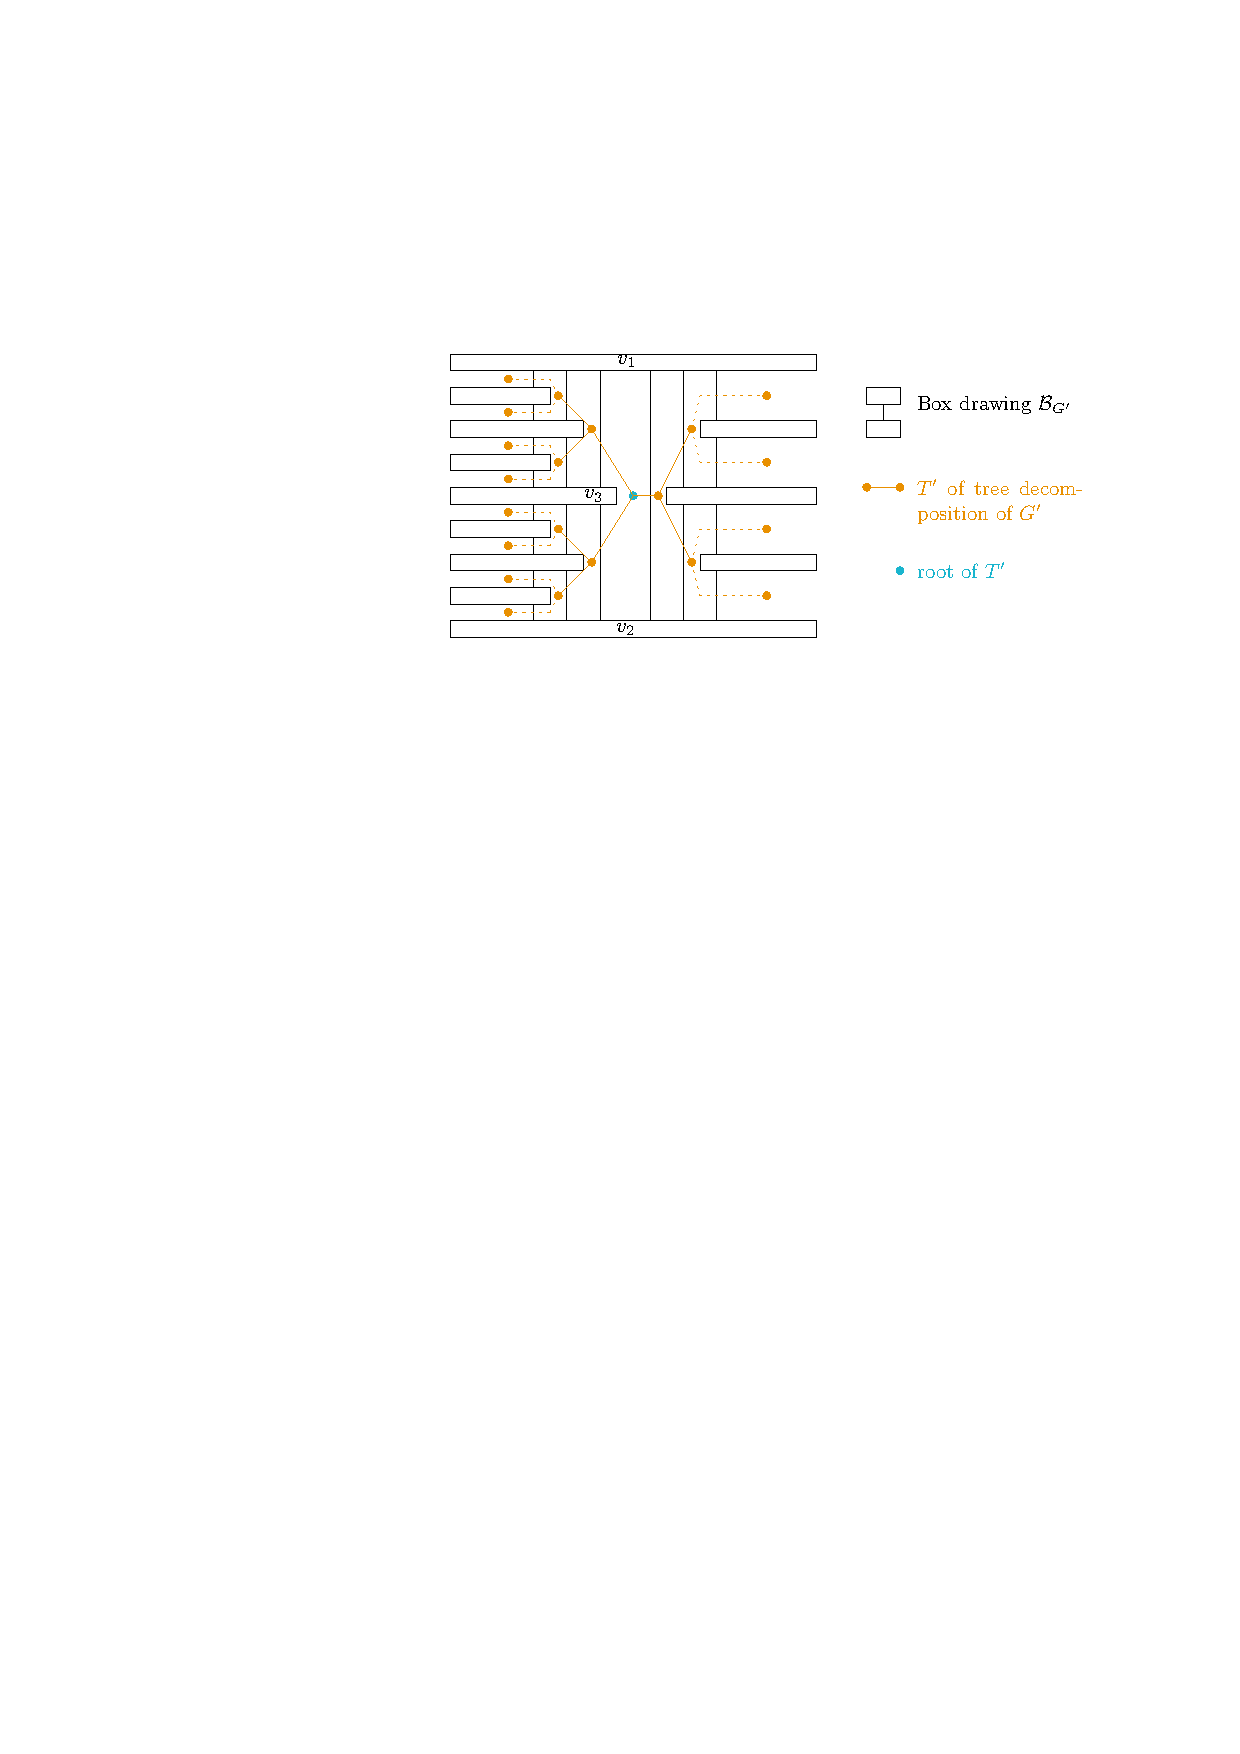
\includegraphics[page=1,width=\linewidth]{graphics/maximal_outerplanar_preserving_outerplanartiy_scheme.pdf}
	\end{subfigure}
	\caption{Scheme to draw a complete maximal outerplanar graph with preserving the outerplanarity property}\label{im:maximal_outerplanar_preserving_outerplanartiy_scheme}
\end{figure}

Since every box of $\mathcal{B}_{G'}$ lies on the outerface, every vertex lies on the outerface in the resulting polyline drawing $\Gamma_{G'}$. The runtime, area consumption and ratio do not alter asymptotically.
\end{proof}
\begin{figure}[H]
	\centering
	\begin{subfigure}{\textwidth}
		\centering
		\includegraphics[page=9,width=0.5\linewidth]{graphics/maximal_outerplanar_example_drawings.pdf}
	\end{subfigure}
	\caption{Alternate box drawing of example illustrated at \ref{im:example_drawing_box_G}, preserving outerplanarity}
\end{figure}